\chapter{Présentation des interfaces}

\section{Introduction}

Ce chapitre illustre le livrable tel qu'il apparaît à l'utilisateur. Les captures ont été réalisées sur l'environnement local (\texttt{http://127.0.0.1:5173}), avec le compte administrateur. Elles correspondent aux écrans du menu principal : connexion, tableau de bord, référentiels, missions, assistant, journal d'activités et administration. L'espace «~Mon profil~» du chauffeur n'est pas reproduit ici : il n'est accessible qu'avec un compte \texttt{DRIVER}.

\section{Connexion}

La figure~\ref{fig:ui-login} montre l'écran public de connexion. L'utilisateur saisit son courriel et son mot de passe. Un bouton unique déclenche l'appel d'authentification. En cas de succès, un jeton JWT est stocké côté client et l'application redirige vers le tableau de bord.

\begin{figure}[htbp]
\centering
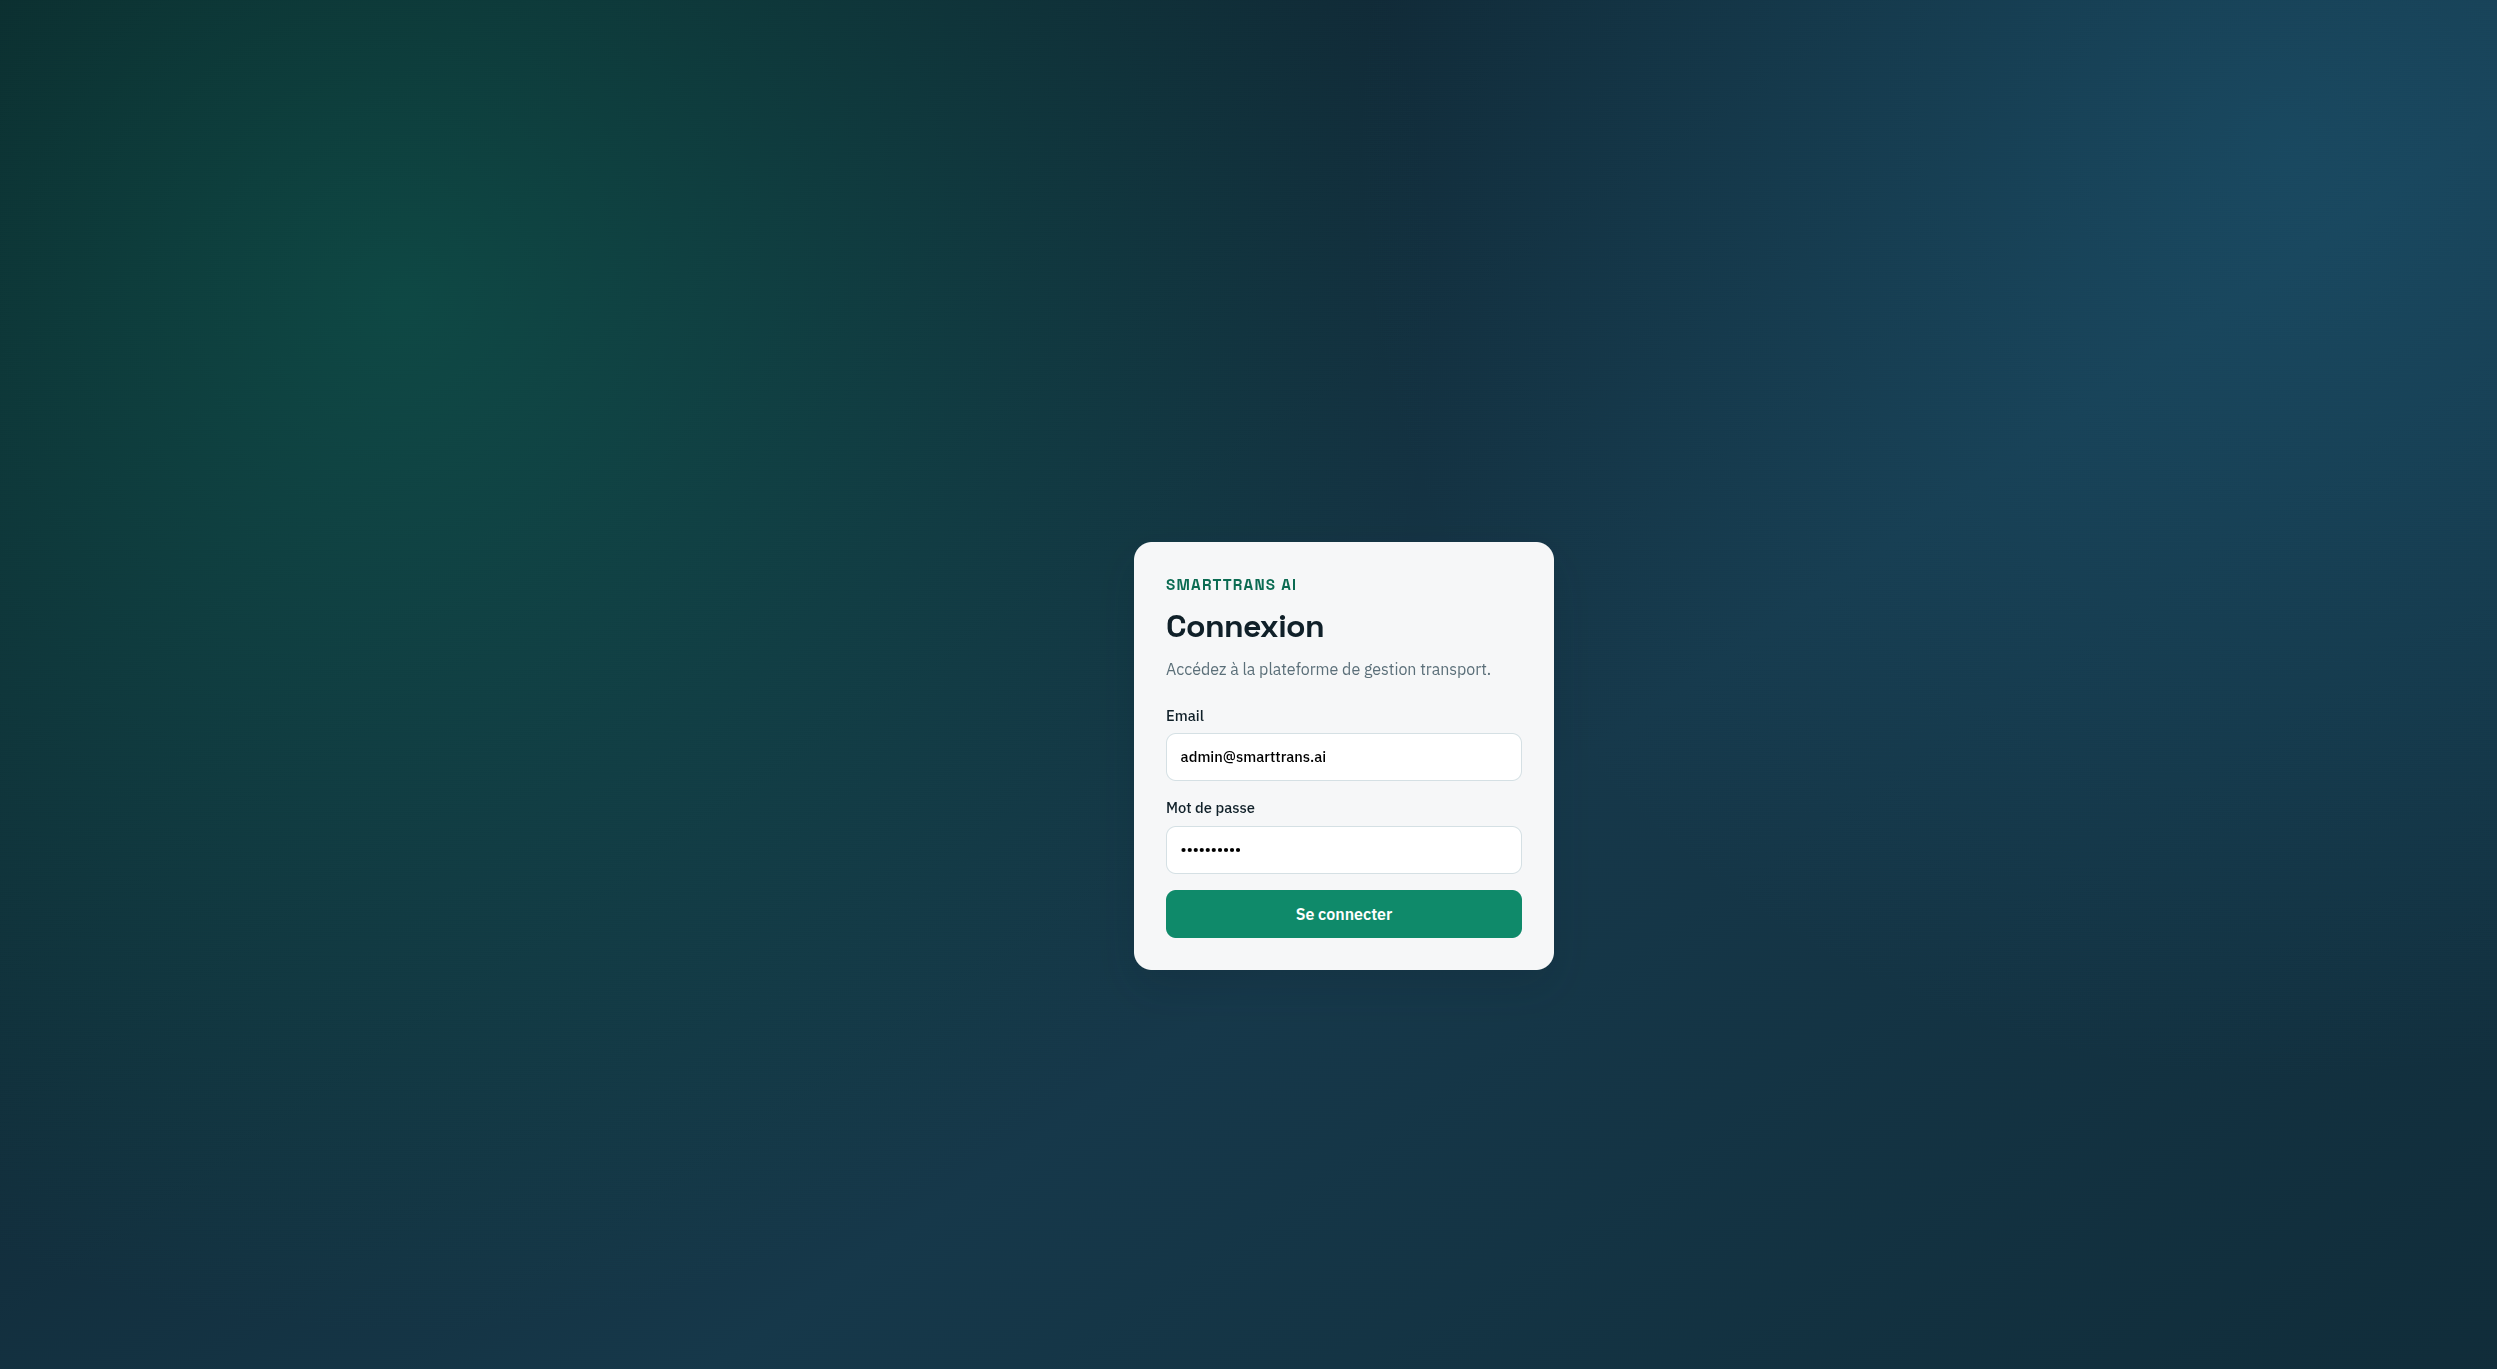
\includegraphics[width=0.82\textwidth,keepaspectratio]{ui-01-login.png}
\caption{Écran de connexion SmartTrans-AI}
\label{fig:ui-login}
\end{figure}

\section{Tableau de bord}

La figure~\ref{fig:ui-dash} présente la vue de pilotage. Les cartes du haut résument les volumes de missions, les ressources disponibles et les alertes (permis, assurance, visite technique). Les graphiques visualisent l'activité de la semaine et la répartition des statuts. Les listes du bas rappellent les prochaines courses, les chauffeurs en mission et les échéances.

\begin{figure}[htbp]
\centering
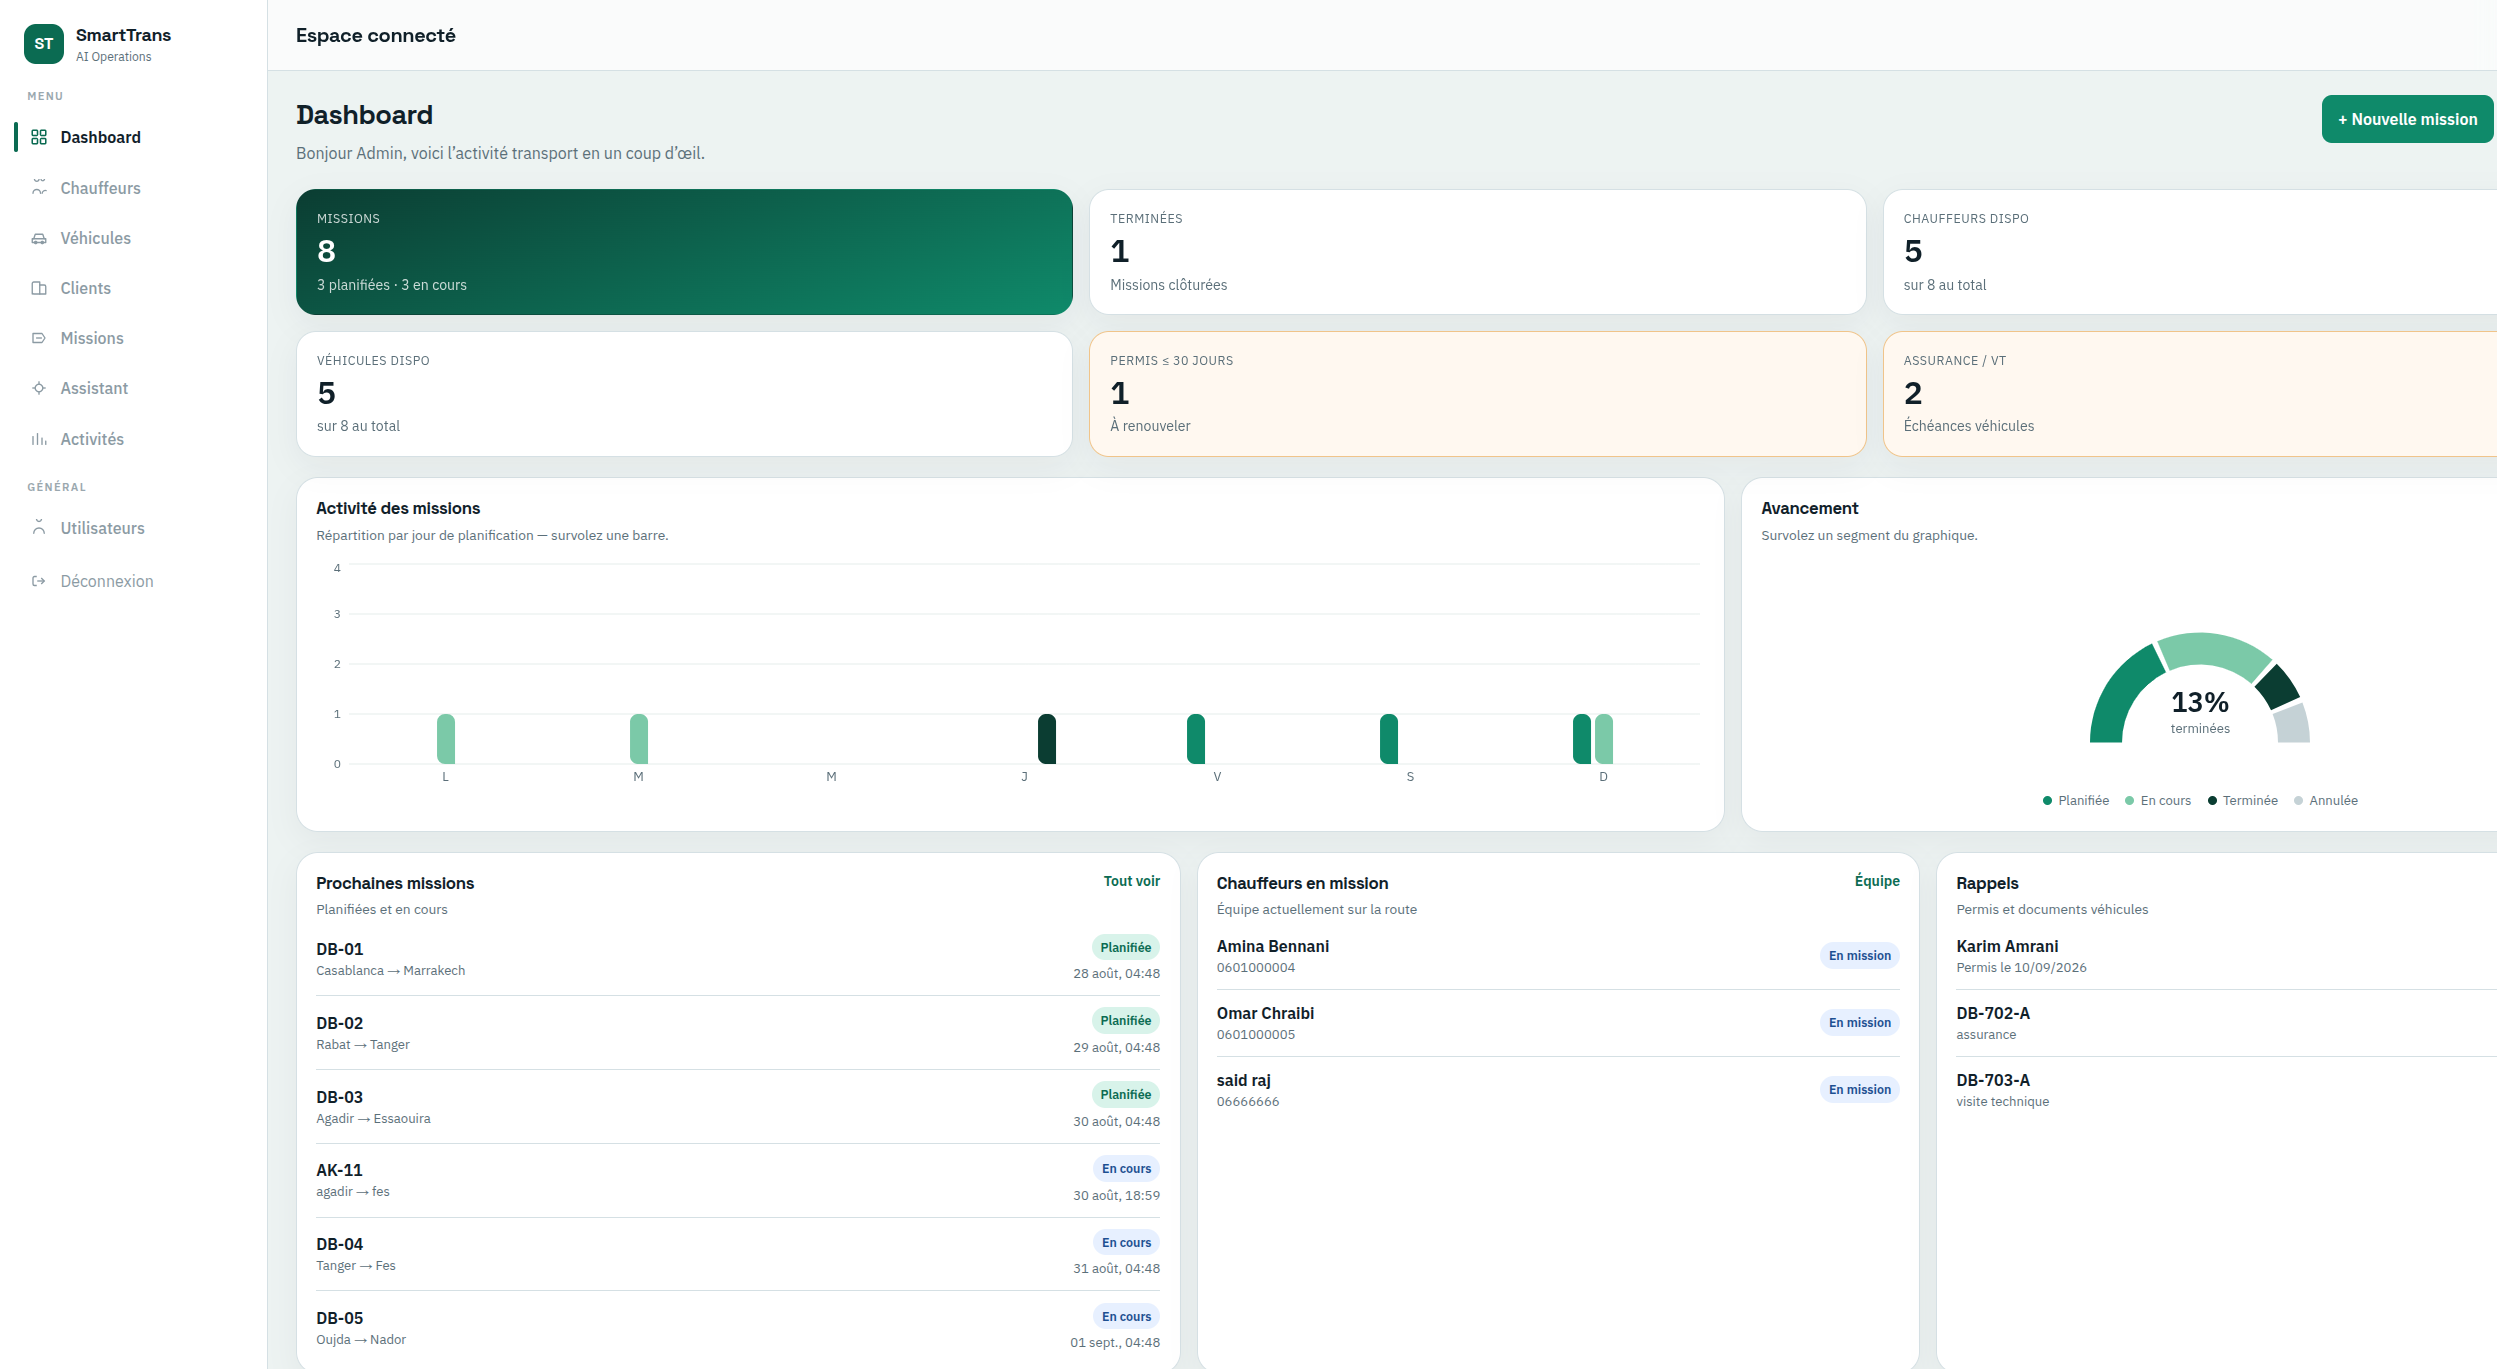
\includegraphics[width=0.95\textwidth,keepaspectratio]{ui-02-dashboard.png}
\caption{Tableau de bord (profil administrateur)}
\label{fig:ui-dash}
\end{figure}

\section{Gestion des chauffeurs}

La liste (figure~\ref{fig:ui-drv-list}) permet de rechercher un chauffeur, de filtrer par statut et par échéance de permis. La création (figure~\ref{fig:ui-drv-new}) saisit l'identité, le permis et le statut. Le détail (figure~\ref{fig:ui-drv-det}) affiche les rappels d'expiration. La modification (figure~\ref{fig:ui-drv-edit}) reprend le même formulaire prérempli.

\begin{figure}[htbp]
\centering
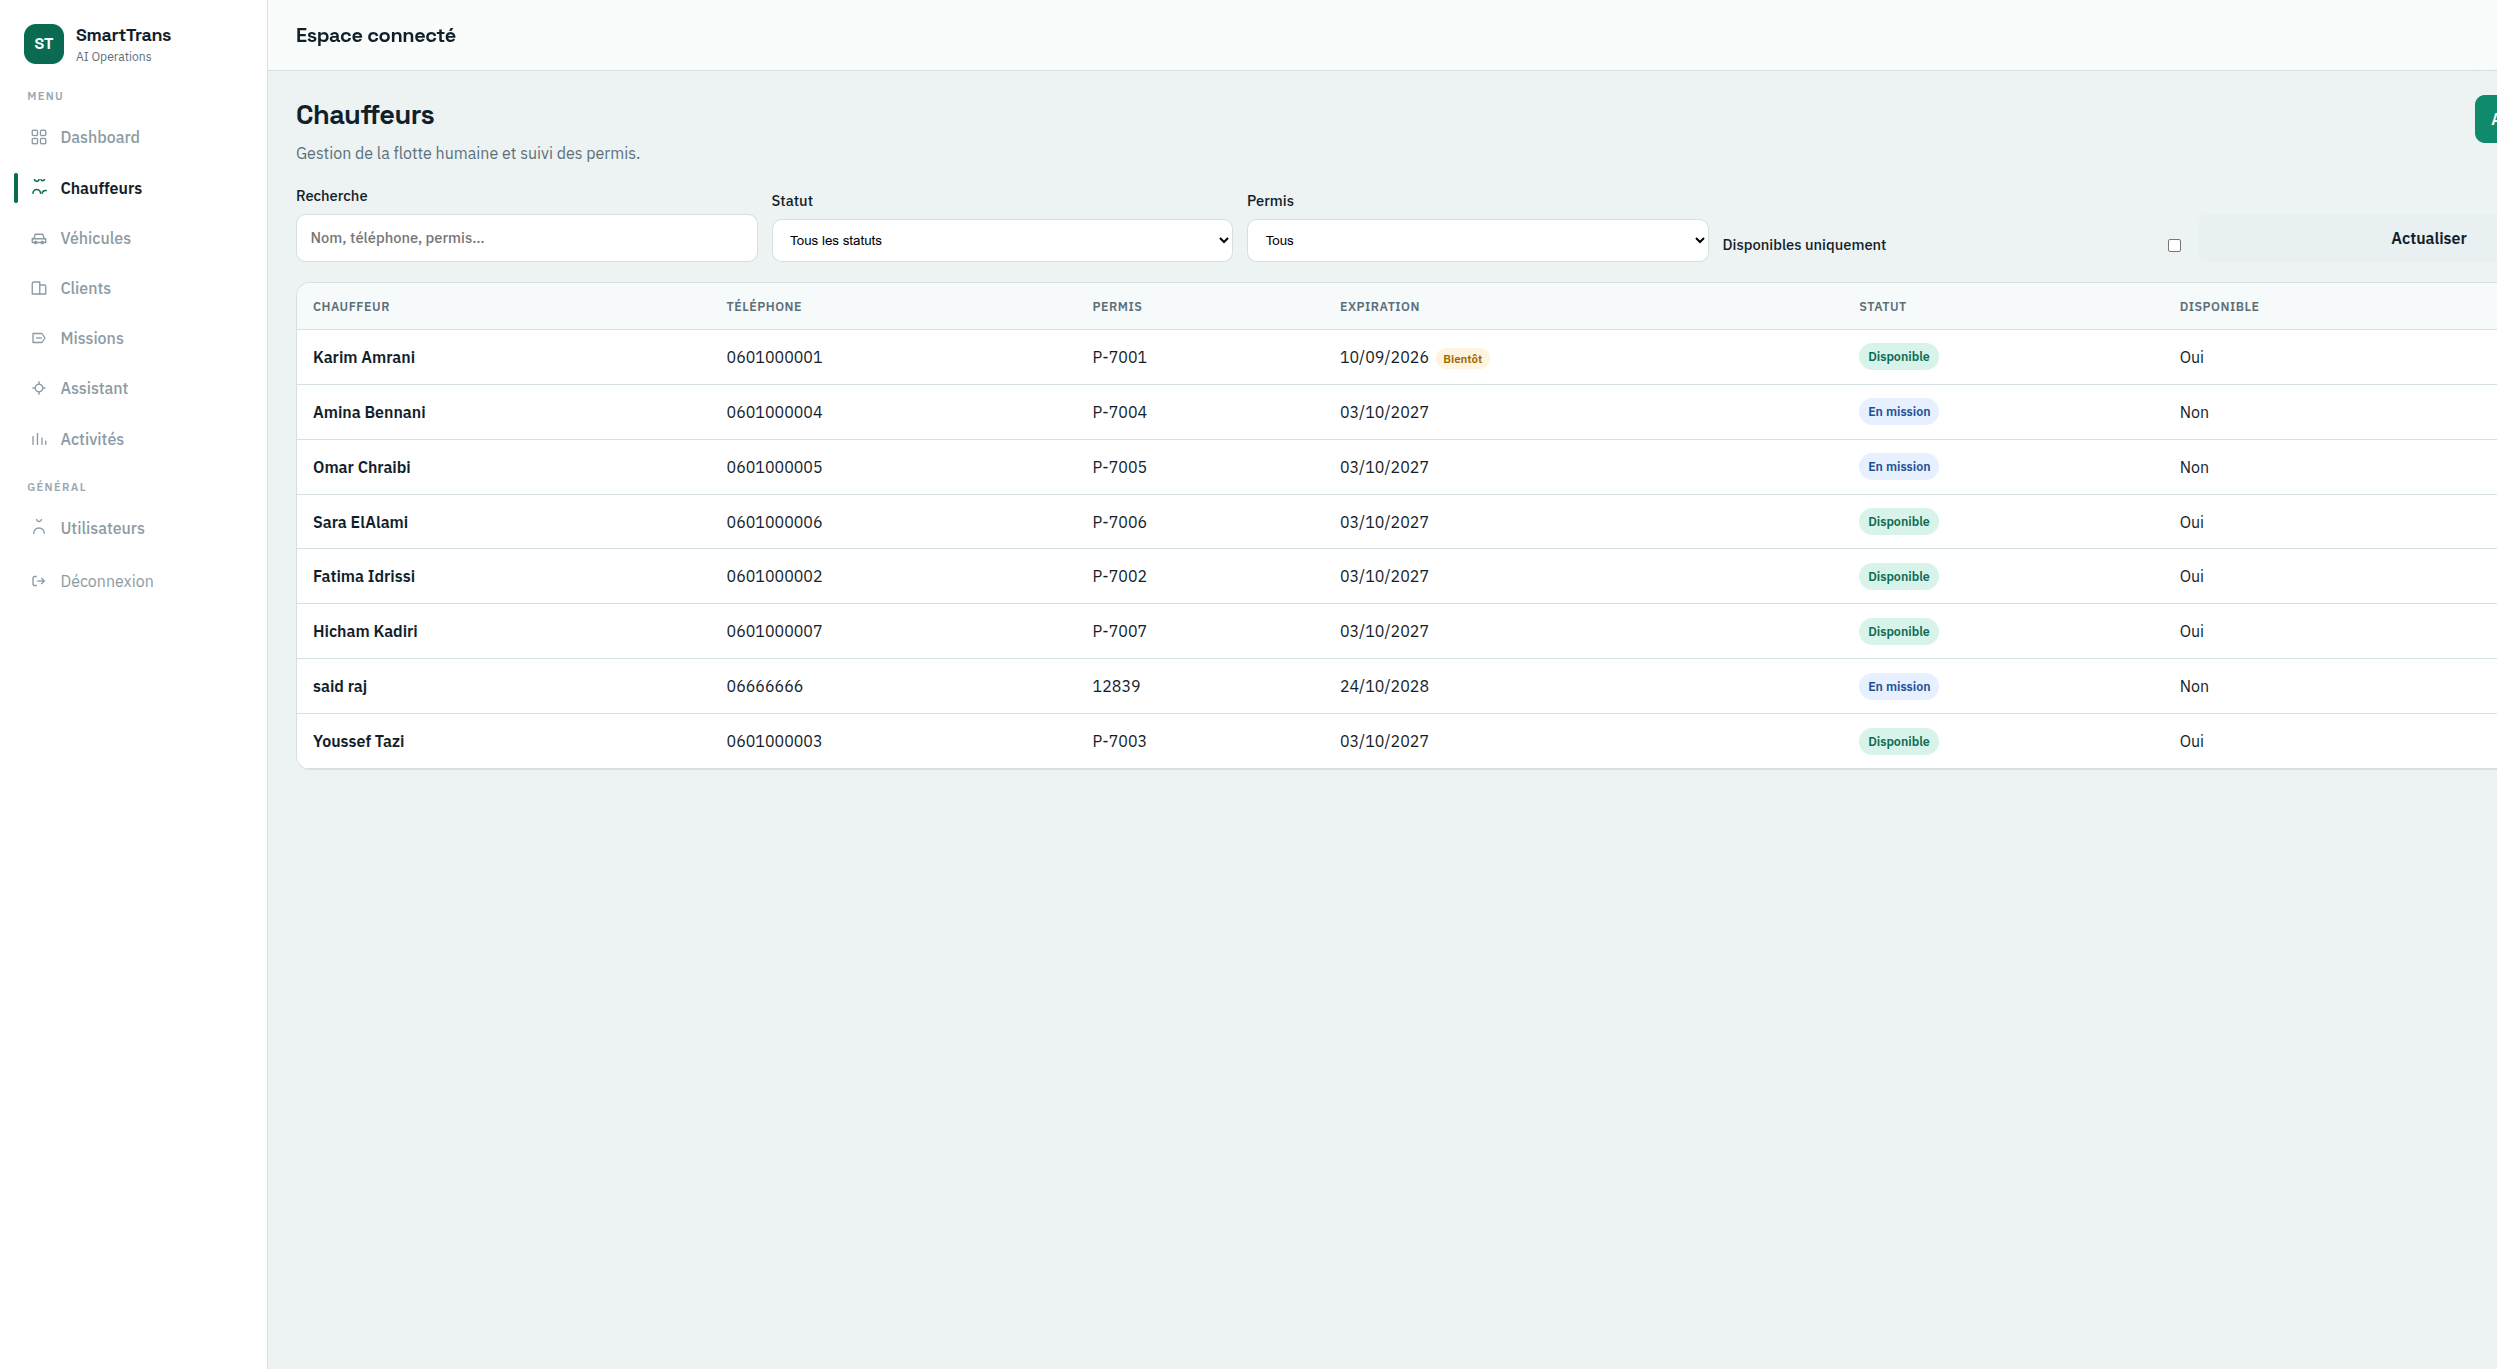
\includegraphics[width=0.95\textwidth,keepaspectratio]{ui-03-chauffeurs.png}
\caption{Liste des chauffeurs}
\label{fig:ui-drv-list}
\end{figure}

\begin{figure}[htbp]
\centering
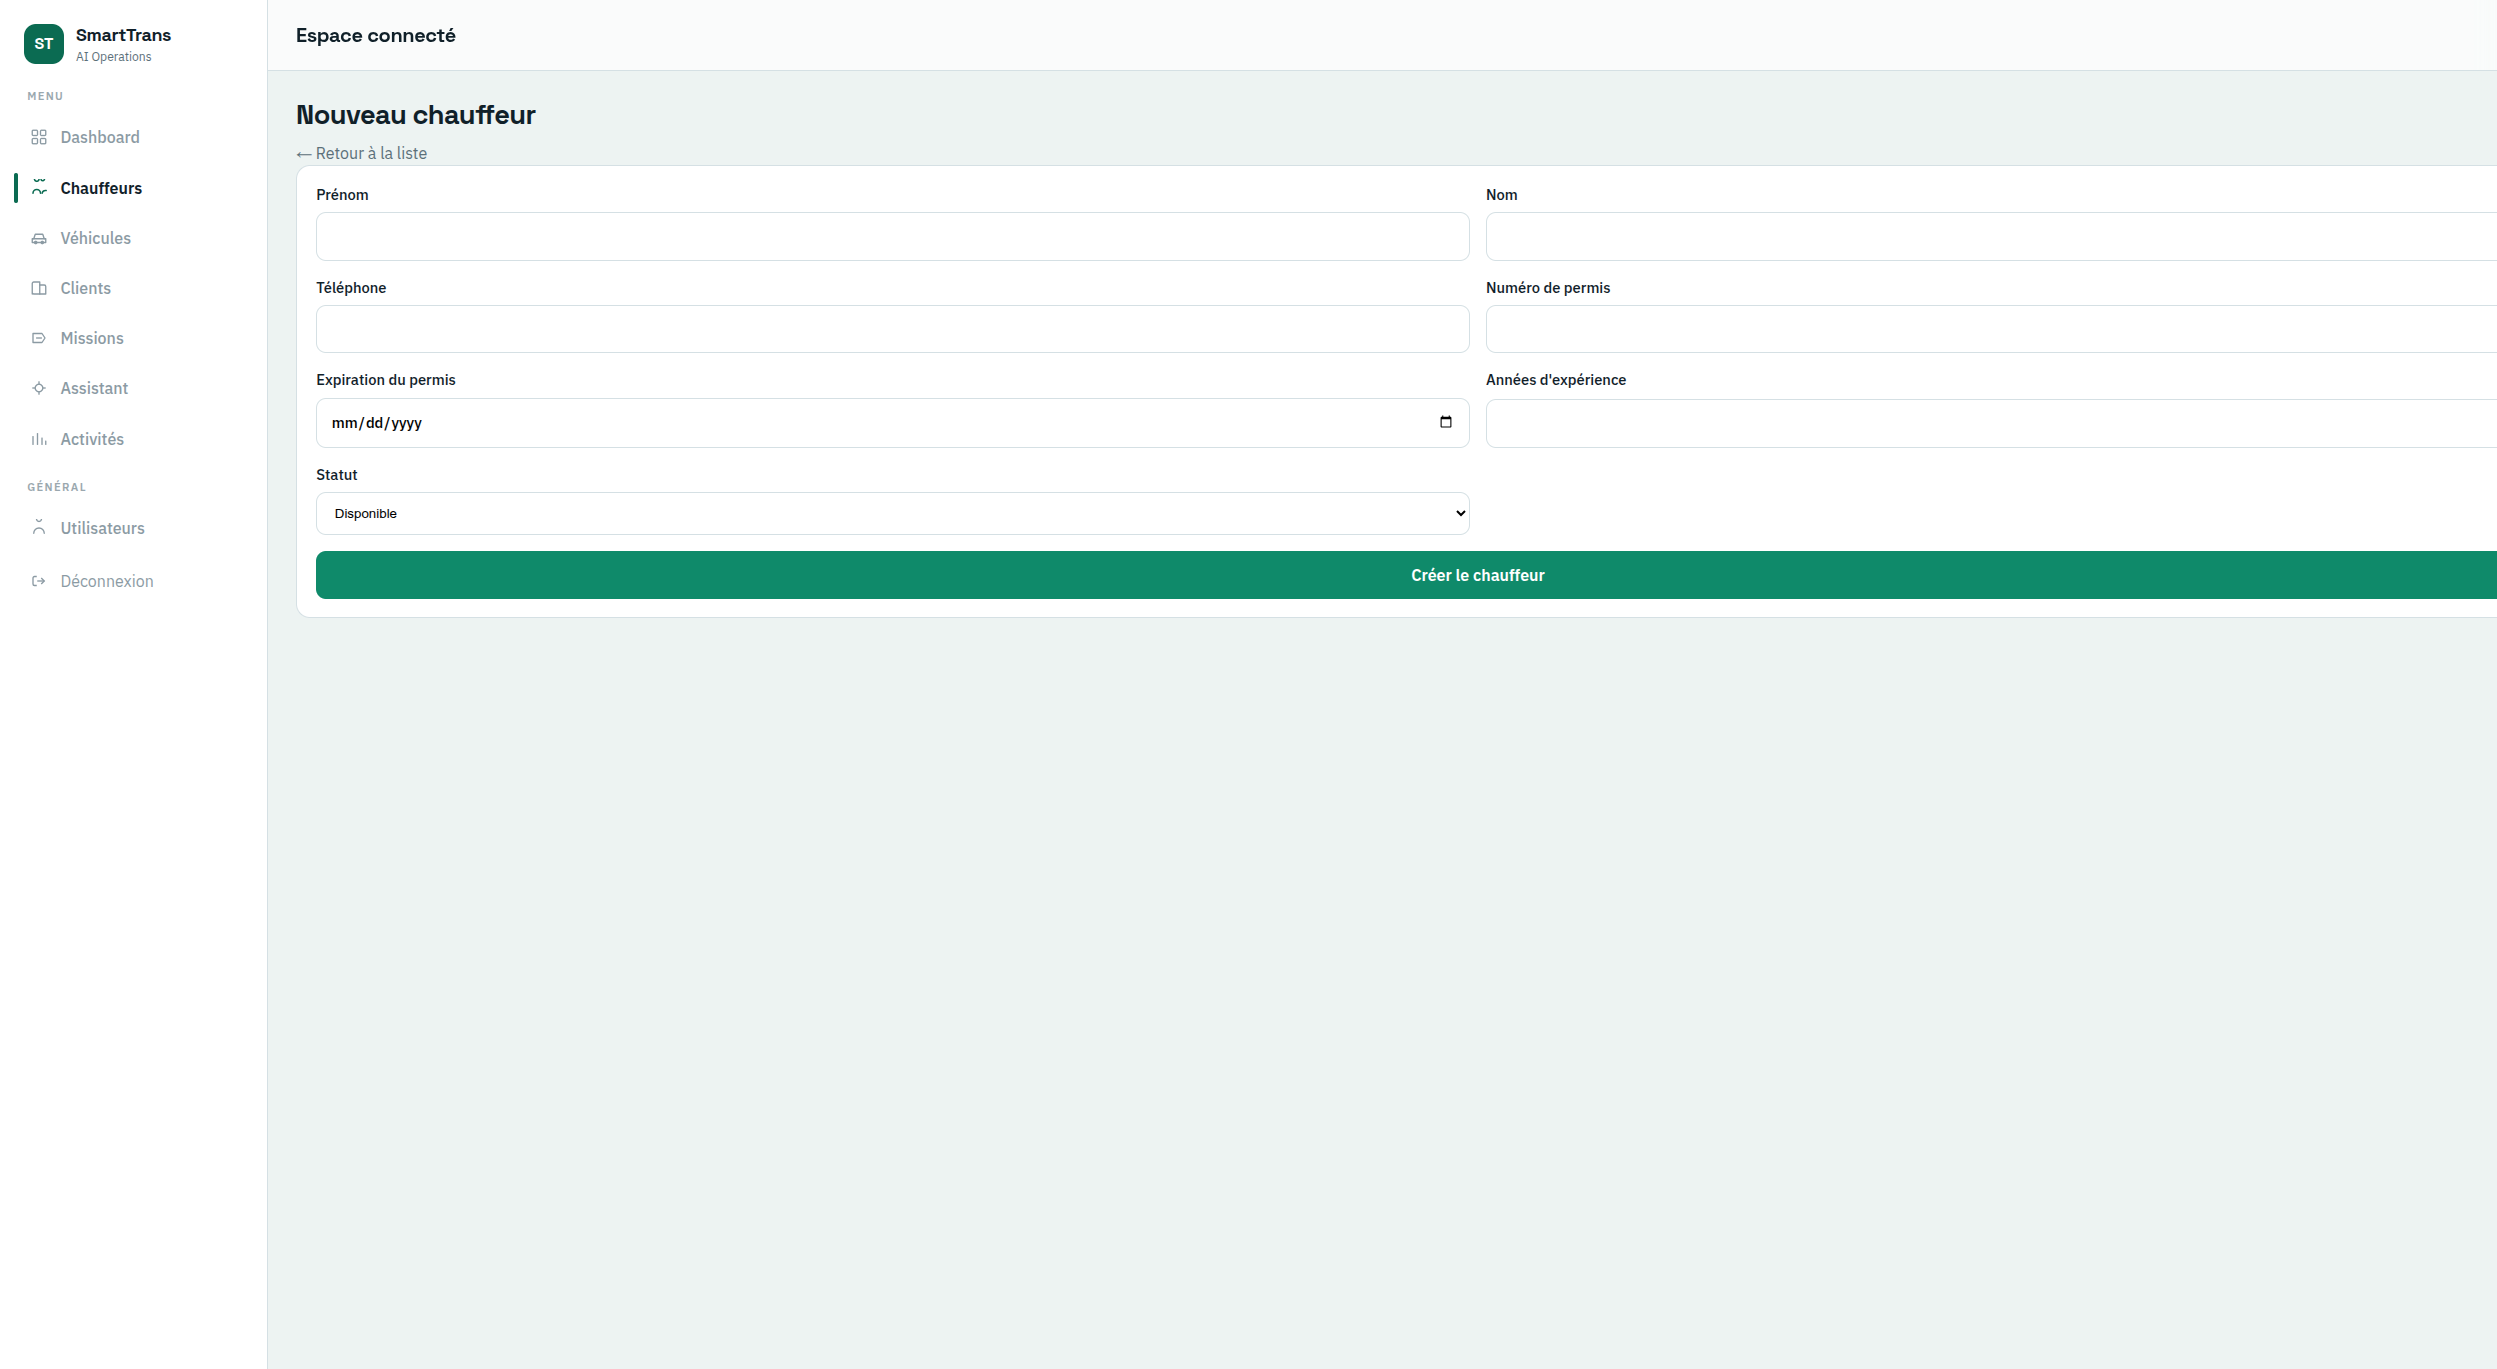
\includegraphics[width=0.88\textwidth,keepaspectratio]{ui-04-chauffeur-nouveau.png}
\caption{Formulaire de création d'un chauffeur}
\label{fig:ui-drv-new}
\end{figure}

\begin{figure}[htbp]
\centering
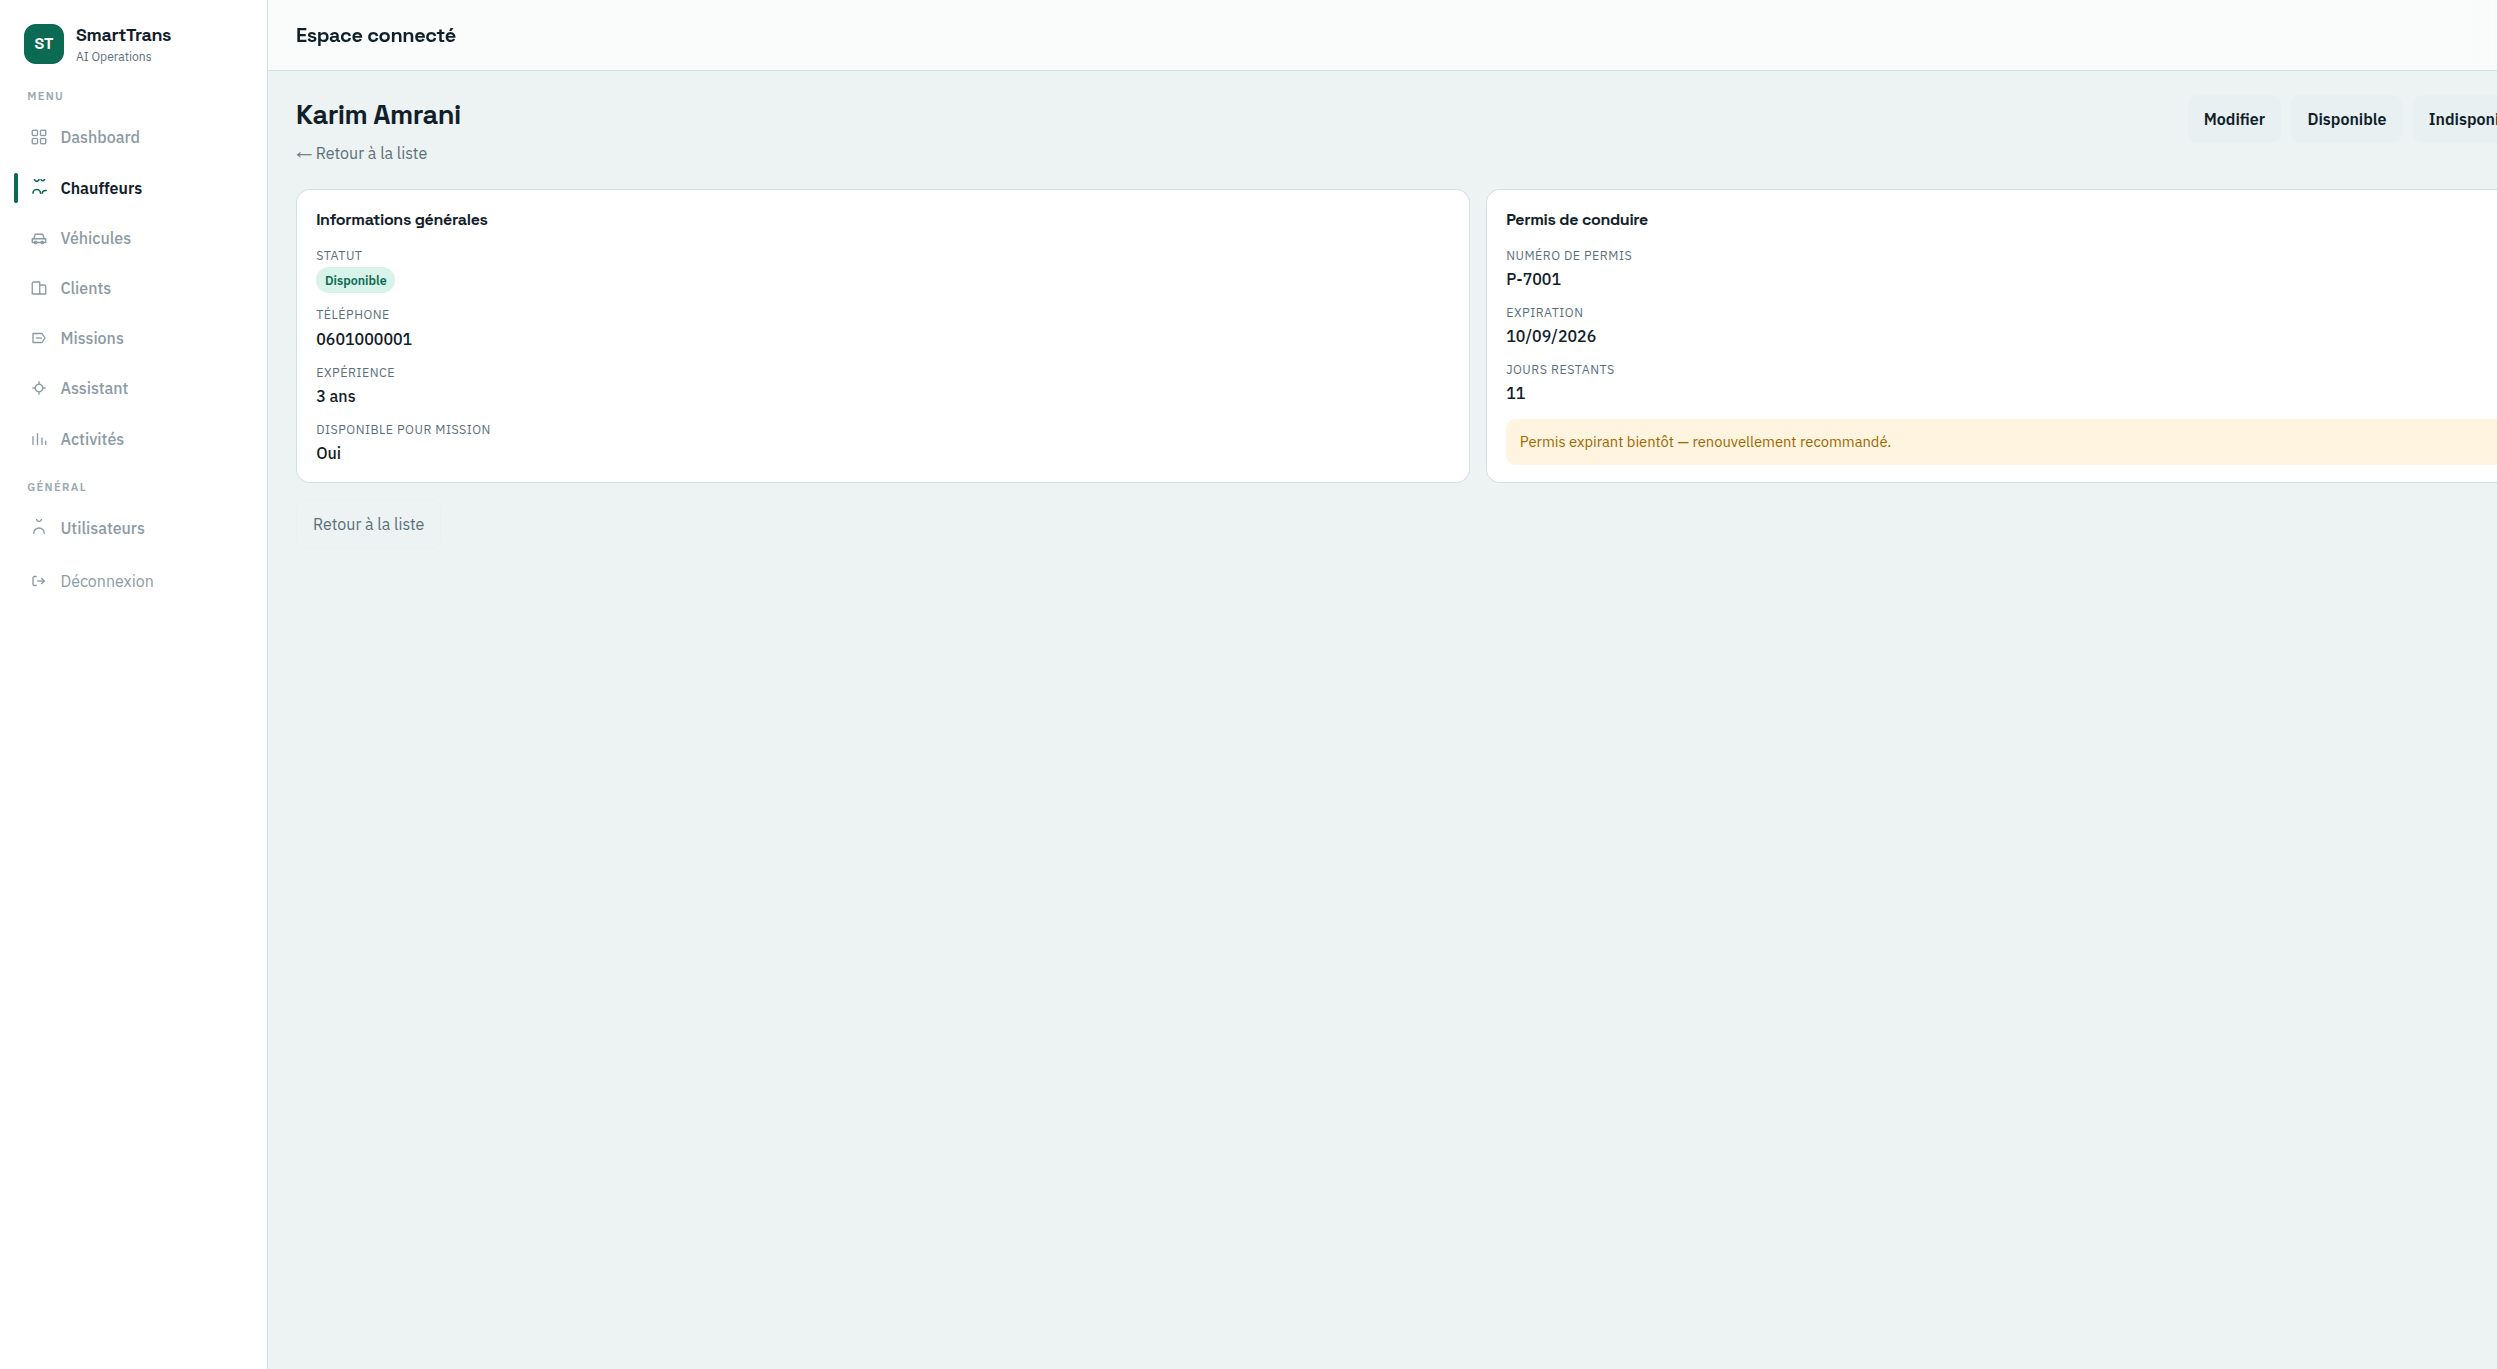
\includegraphics[width=0.88\textwidth,keepaspectratio]{ui-05-chauffeur-detail.png}
\caption{Fiche détail d'un chauffeur (alerte permis)}
\label{fig:ui-drv-det}
\end{figure}

\begin{figure}[htbp]
\centering
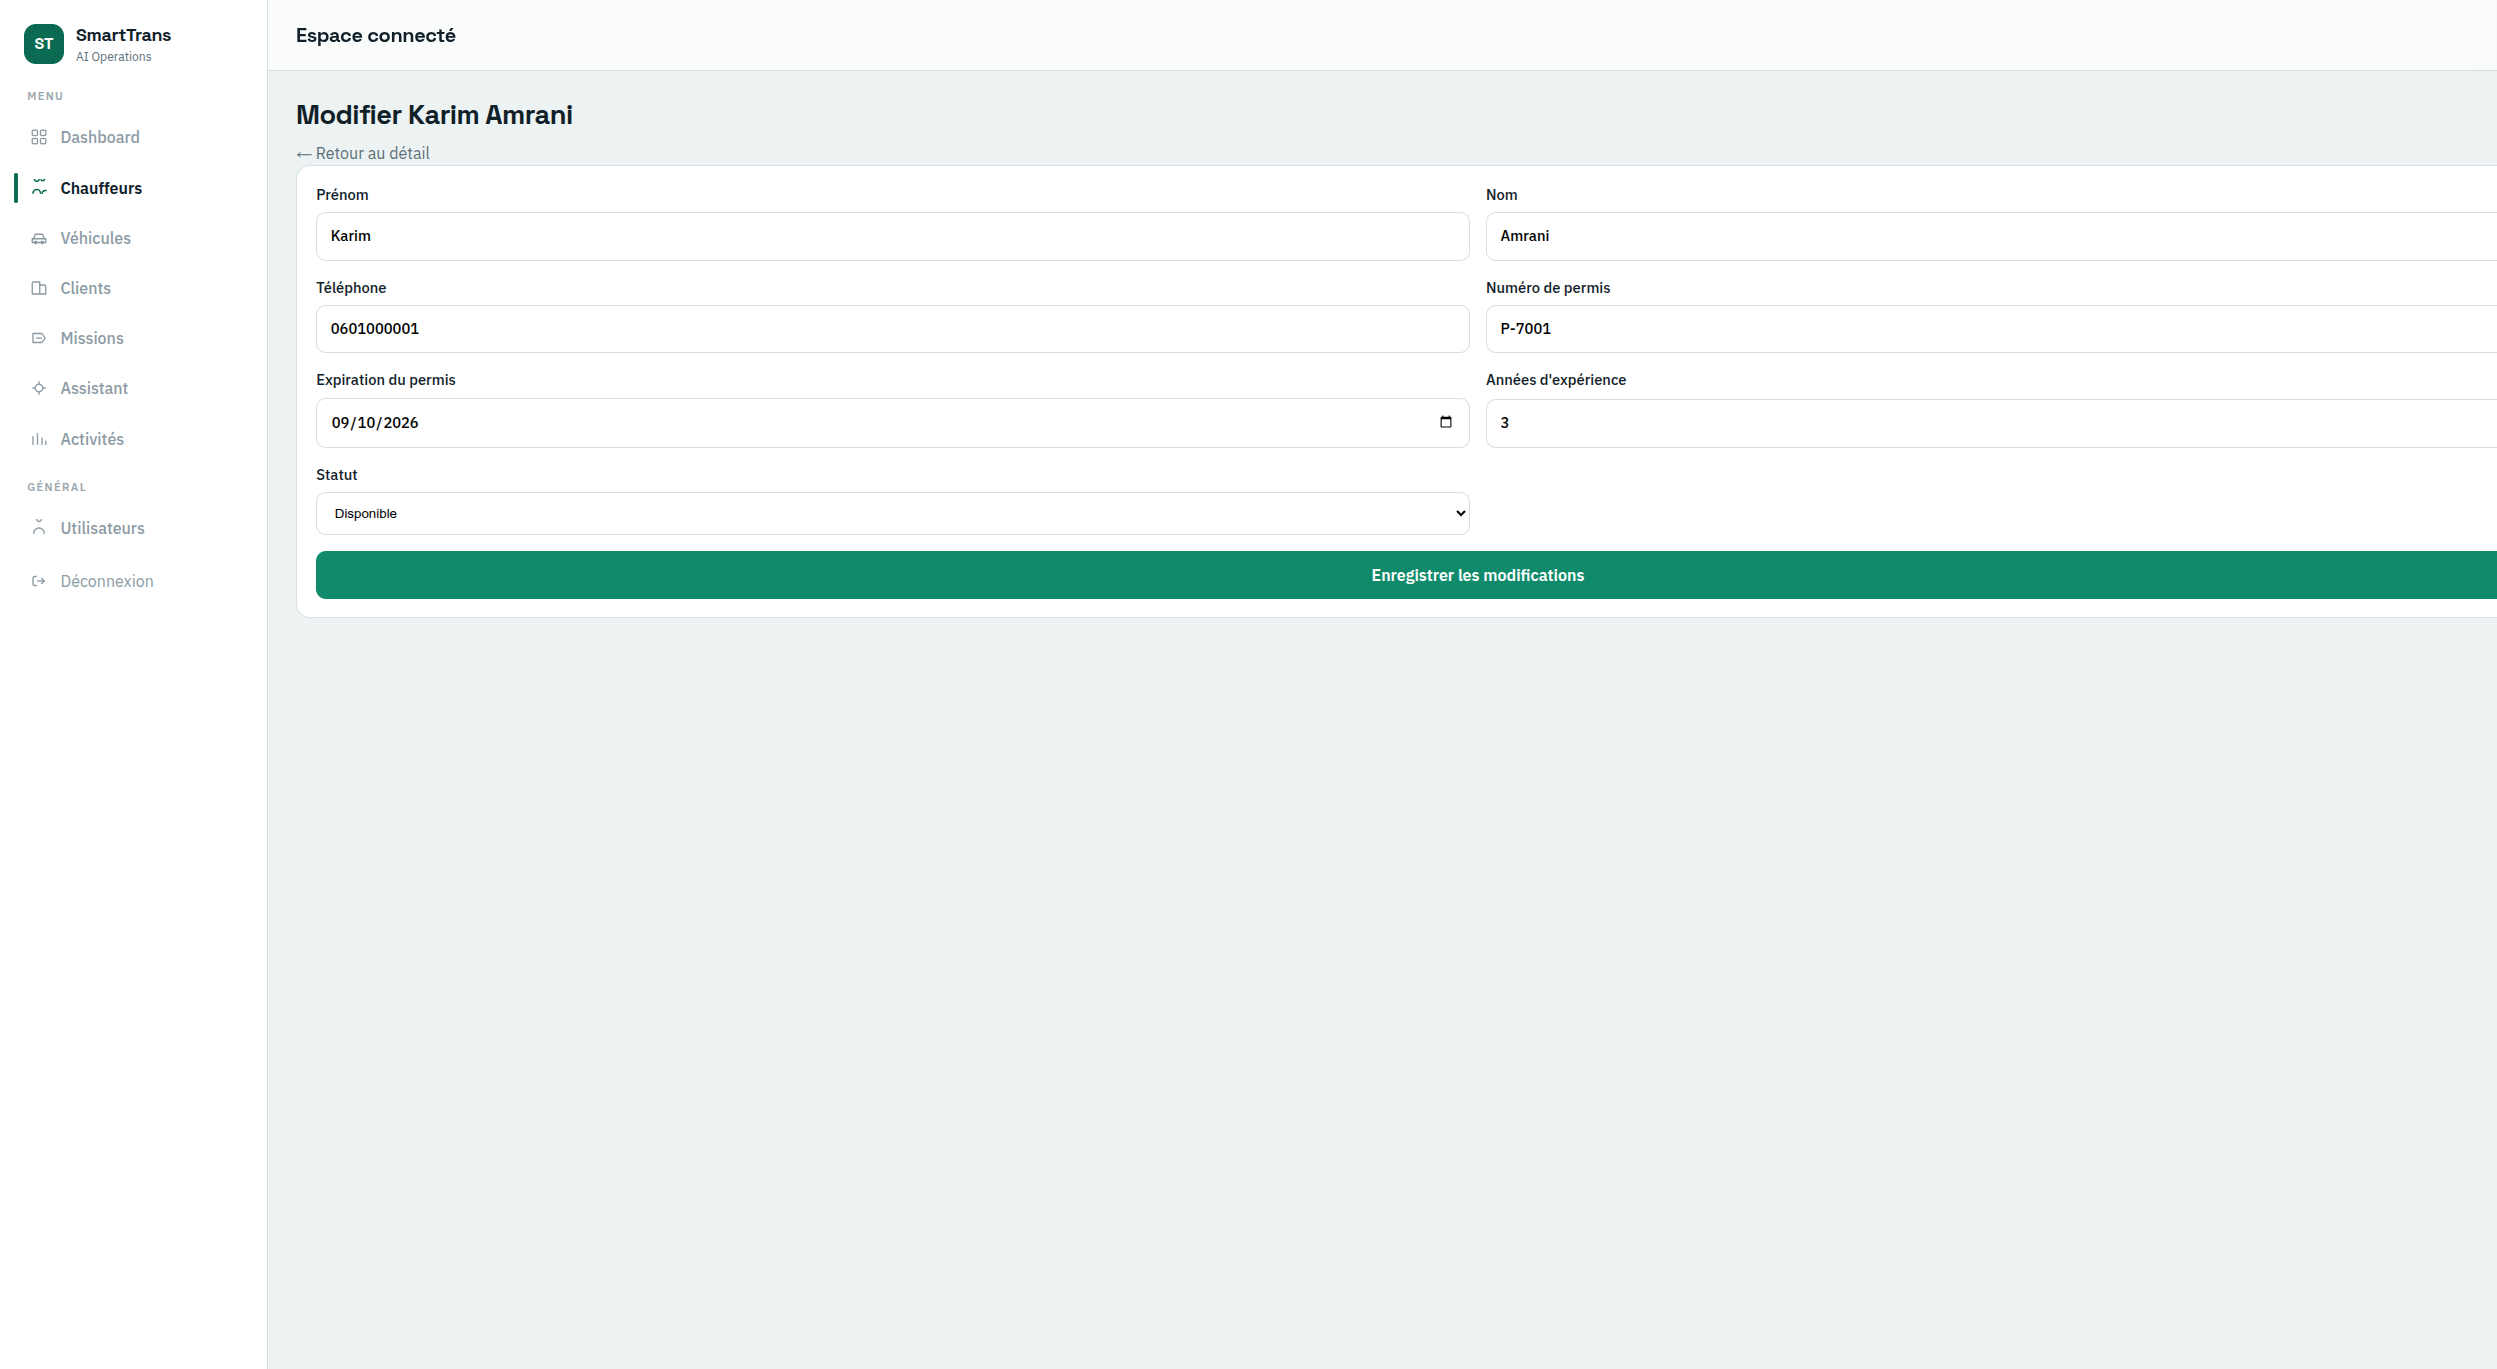
\includegraphics[width=0.88\textwidth,keepaspectratio]{ui-06-chauffeur-edit.png}
\caption{Formulaire de modification d'un chauffeur}
\label{fig:ui-drv-edit}
\end{figure}

\section{Gestion des véhicules}

La liste (figure~\ref{fig:ui-veh-list}) suit immatriculation, type, kilométrage, dates d'assurance et de visite technique, et statut d'exploitation. Le formulaire de création (figure~\ref{fig:ui-veh-new}) et la fiche détail (figure~\ref{fig:ui-veh-det}) reprennent ces champs, avec un indicateur de validité des documents.

\begin{figure}[htbp]
\centering
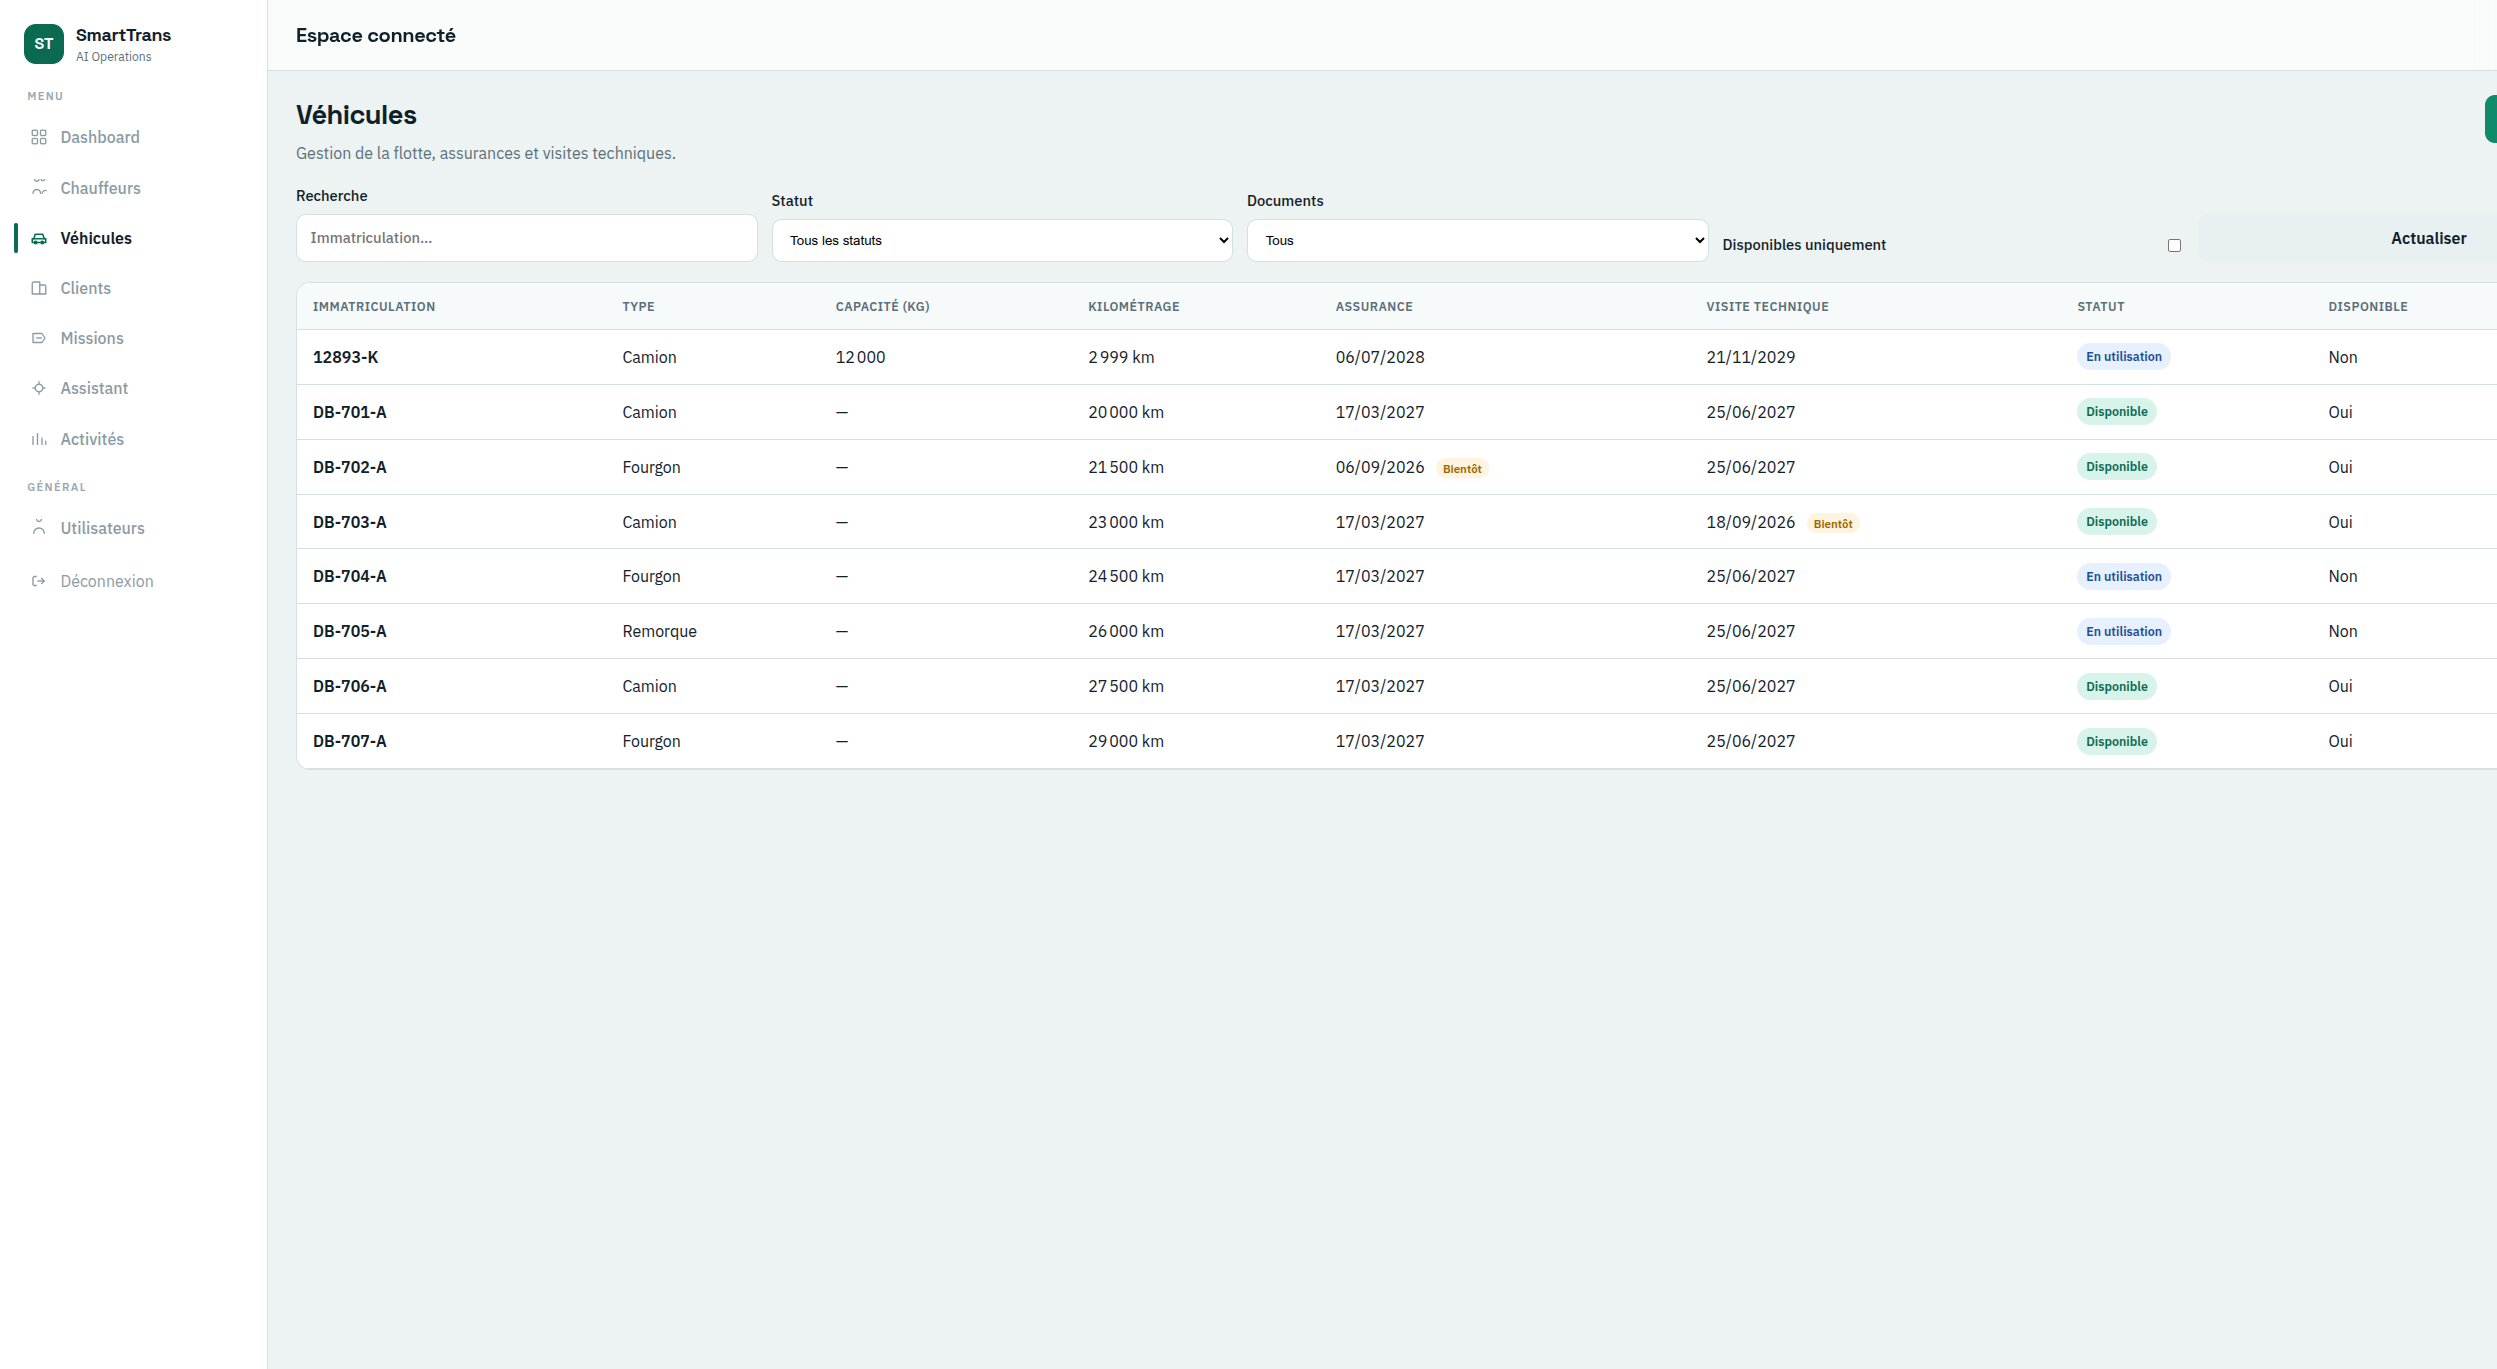
\includegraphics[width=0.95\textwidth,keepaspectratio]{ui-07-vehicules.png}
\caption{Liste des véhicules}
\label{fig:ui-veh-list}
\end{figure}

\begin{figure}[htbp]
\centering
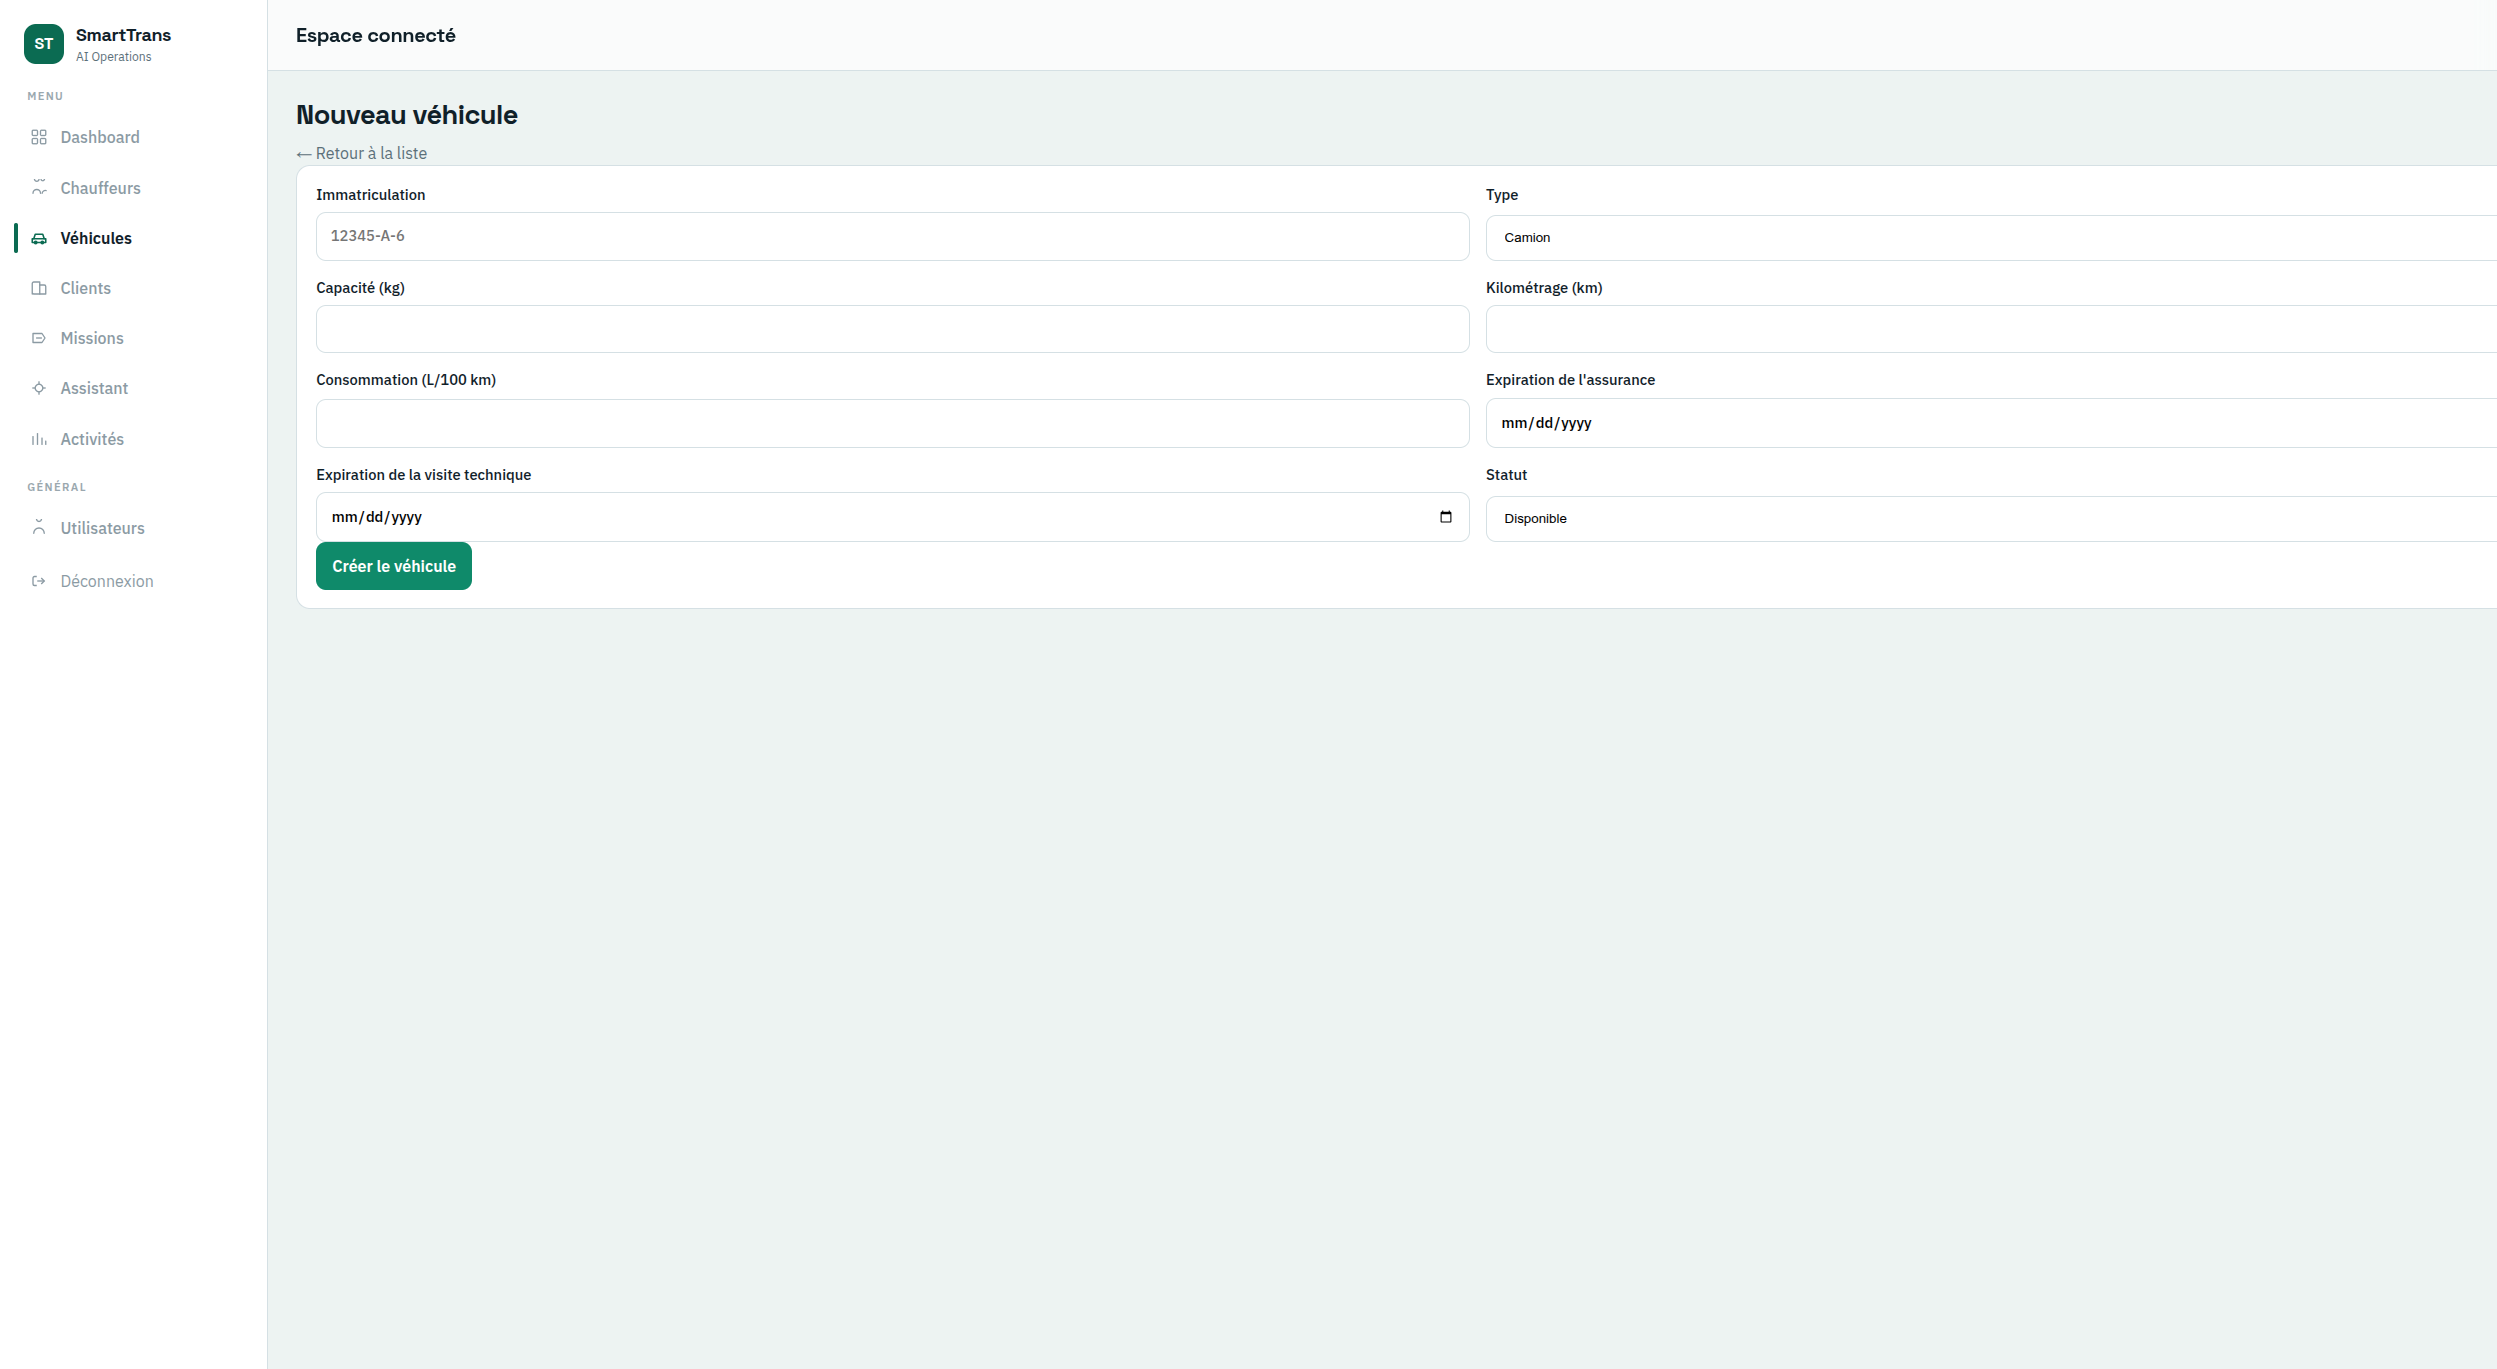
\includegraphics[width=0.88\textwidth,keepaspectratio]{ui-08-vehicule-nouveau.png}
\caption{Formulaire de création d'un véhicule}
\label{fig:ui-veh-new}
\end{figure}

\begin{figure}[htbp]
\centering
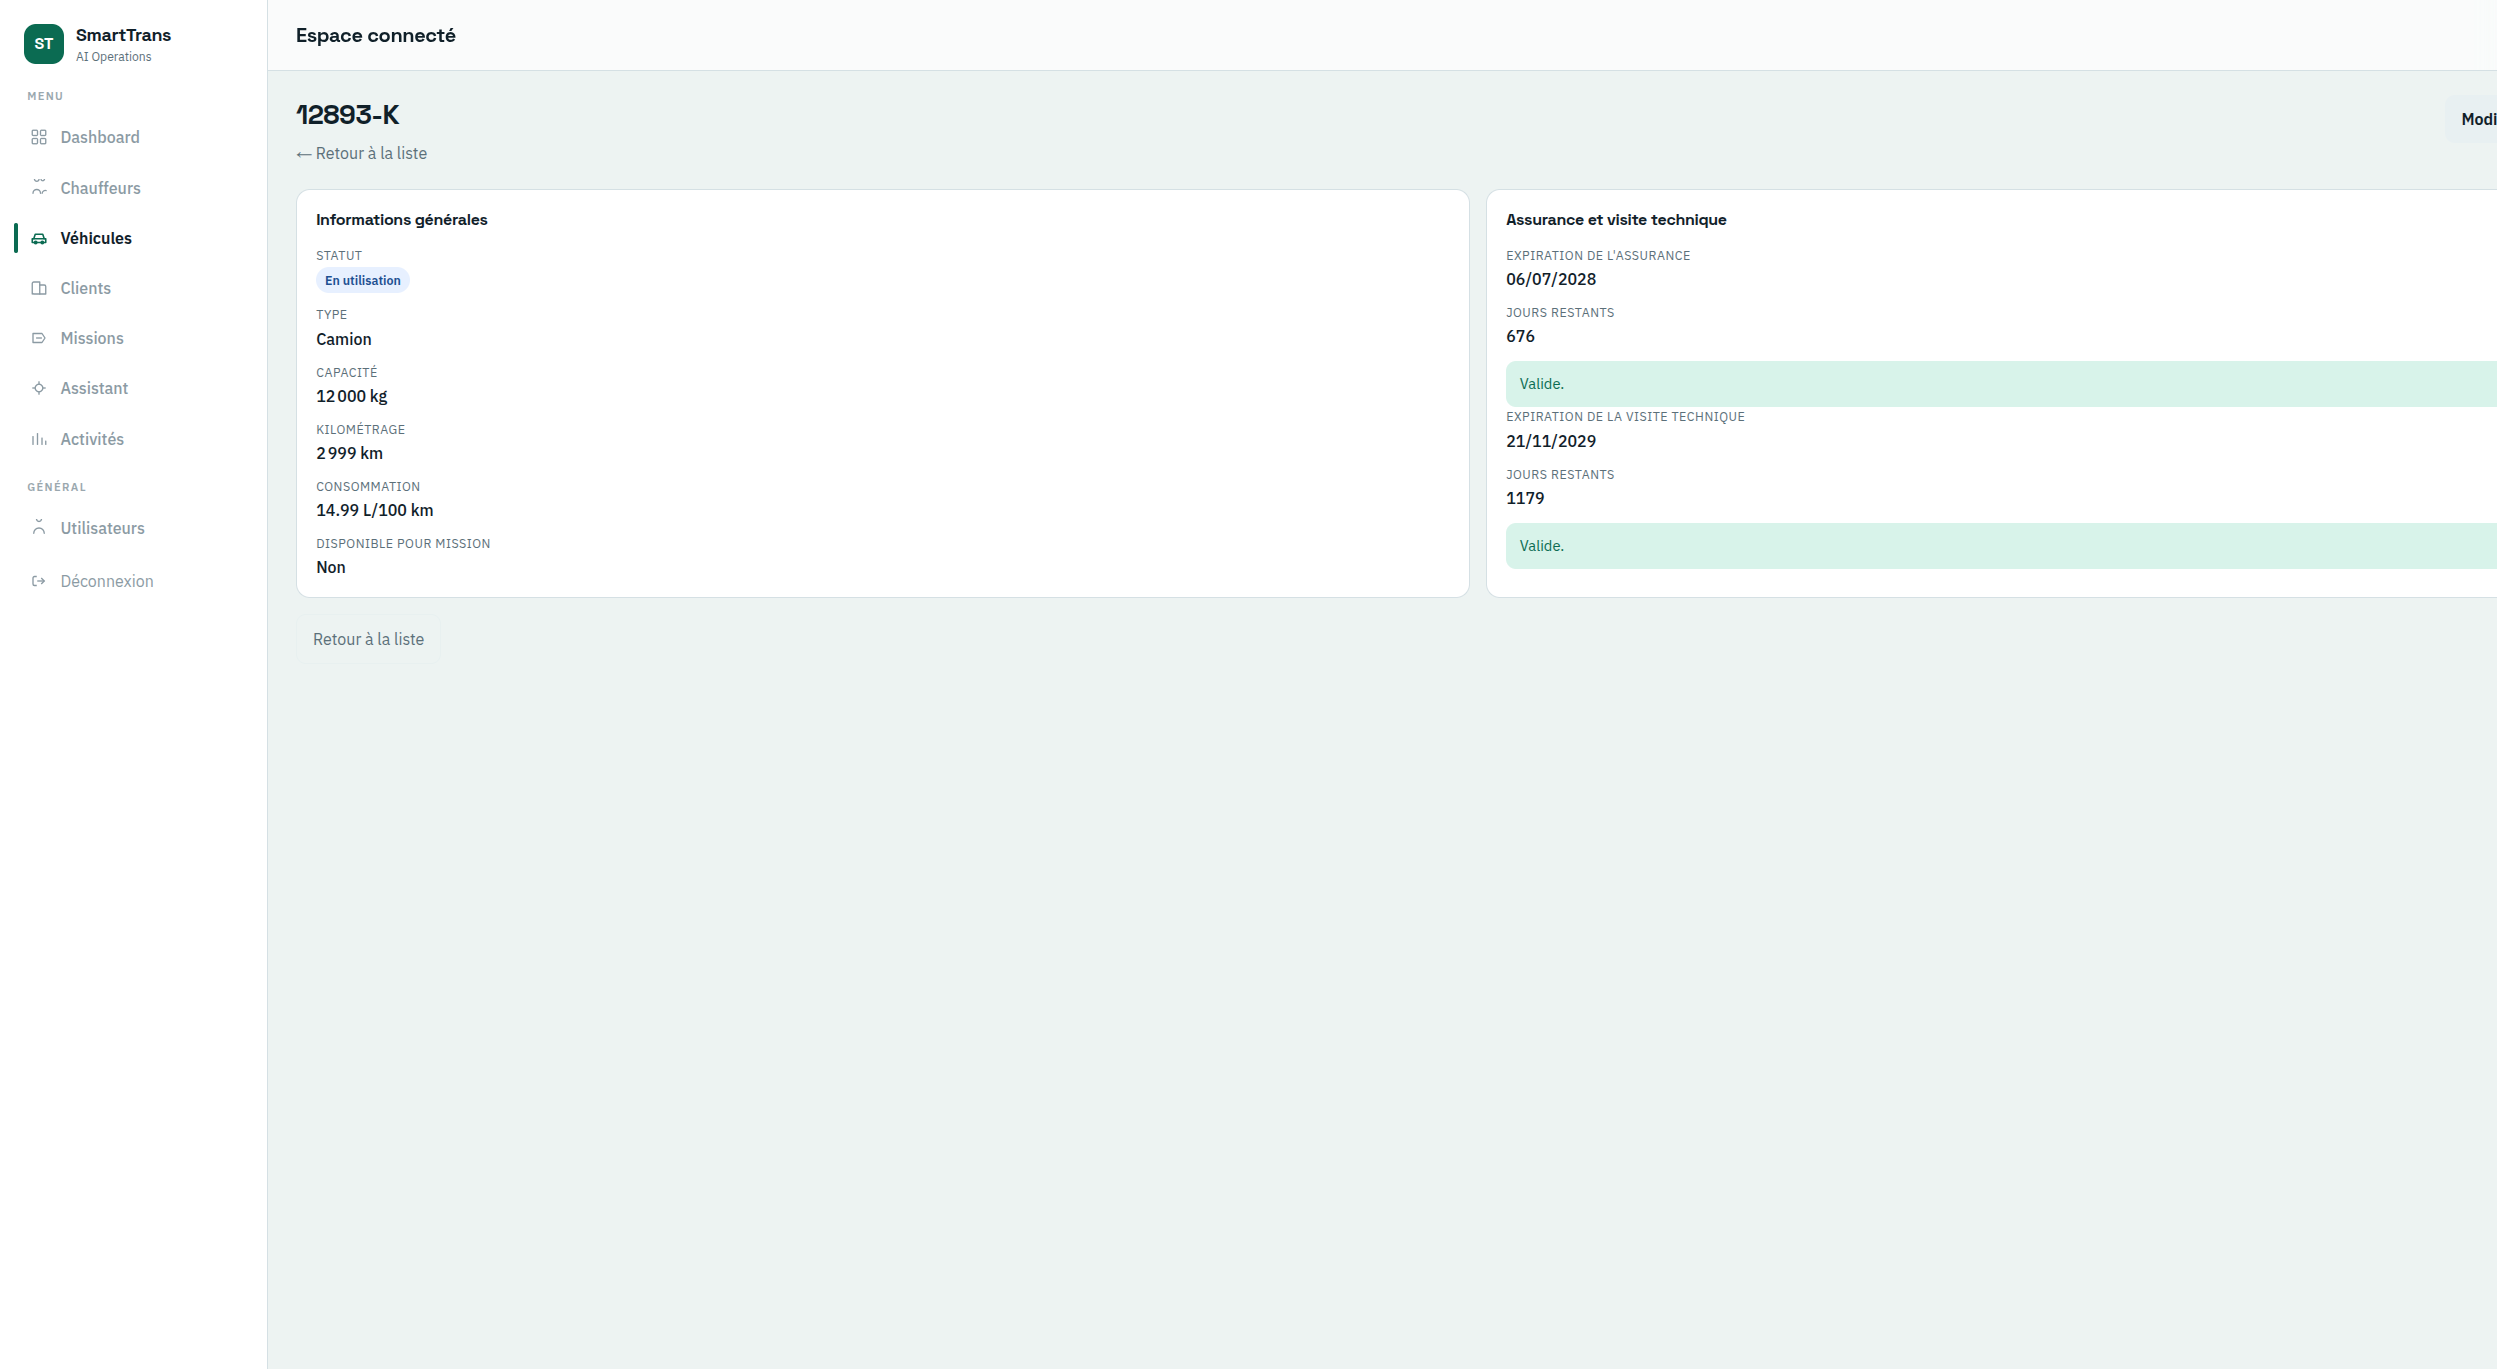
\includegraphics[width=0.88\textwidth,keepaspectratio]{ui-09-vehicule-detail.png}
\caption{Fiche détail d'un véhicule}
\label{fig:ui-veh-det}
\end{figure}

\section{Gestion des clients}

Les clients sont les entreprises destinataires des missions. La liste (figure~\ref{fig:ui-cli-list}) affiche le nom de l'entreprise, les coordonnées et l'adresse. La création (figure~\ref{fig:ui-cli-new}) et le détail (figure~\ref{fig:ui-cli-det}) correspondent à ce référentiel, obligatoire à la planification d'une mission.

\begin{figure}[htbp]
\centering
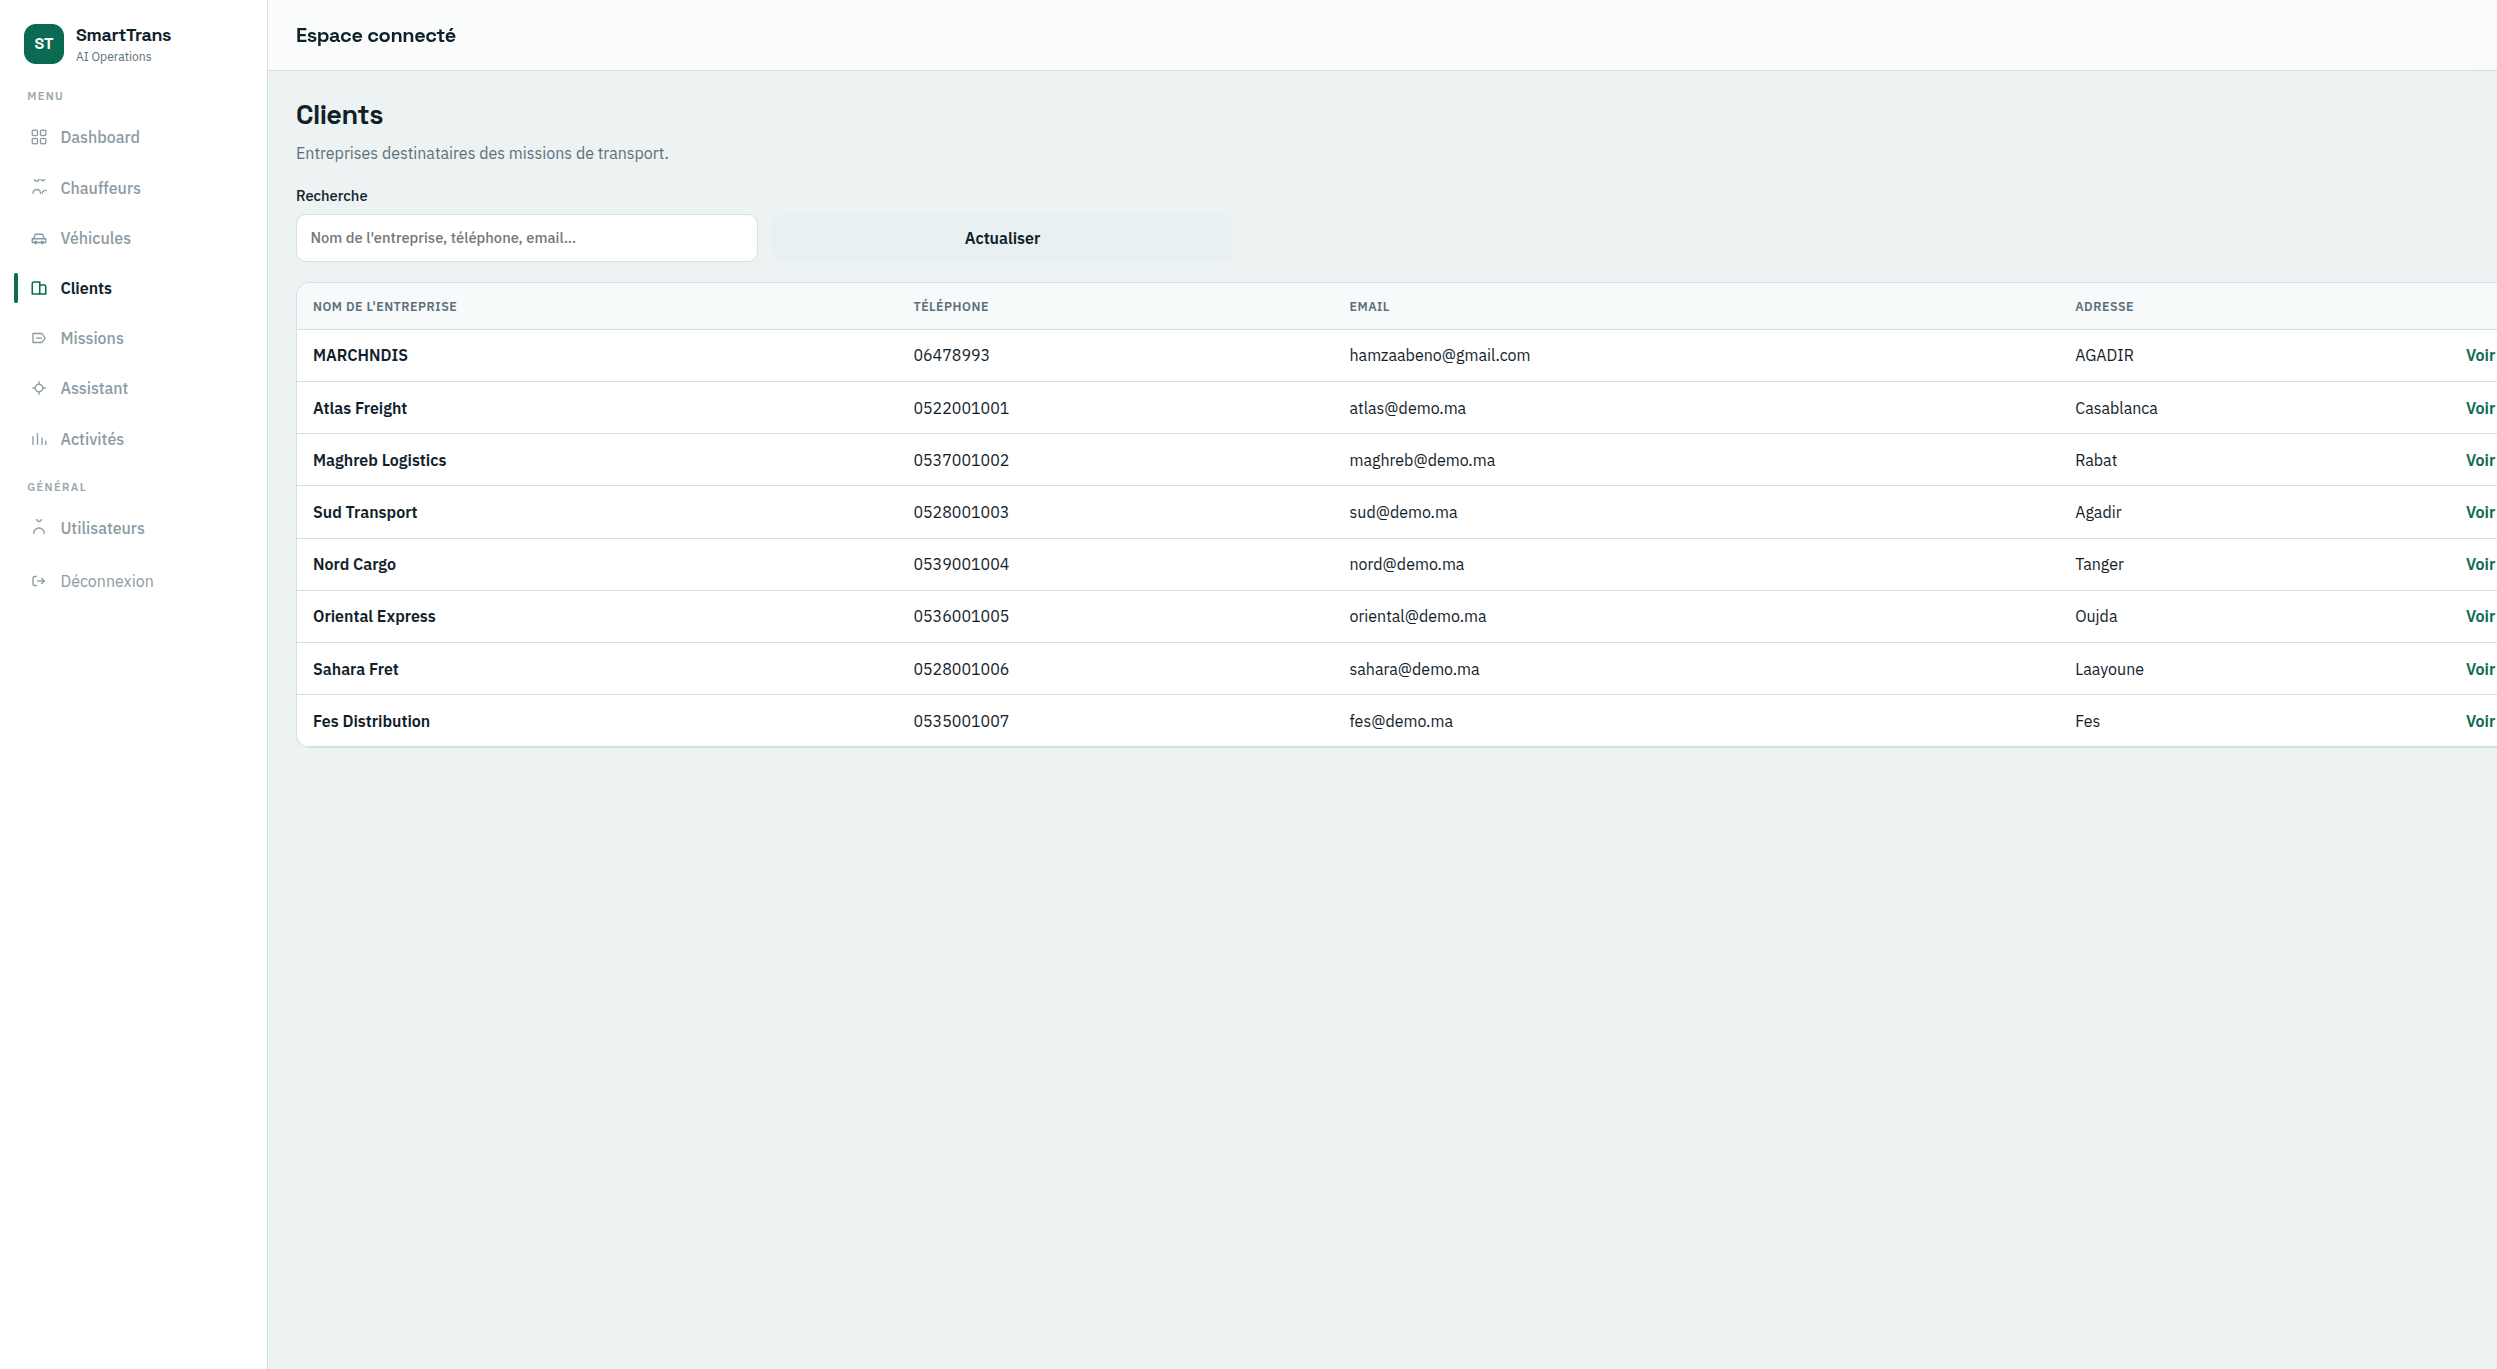
\includegraphics[width=0.95\textwidth,keepaspectratio]{ui-10-clients.png}
\caption{Liste des clients}
\label{fig:ui-cli-list}
\end{figure}

\begin{figure}[htbp]
\centering
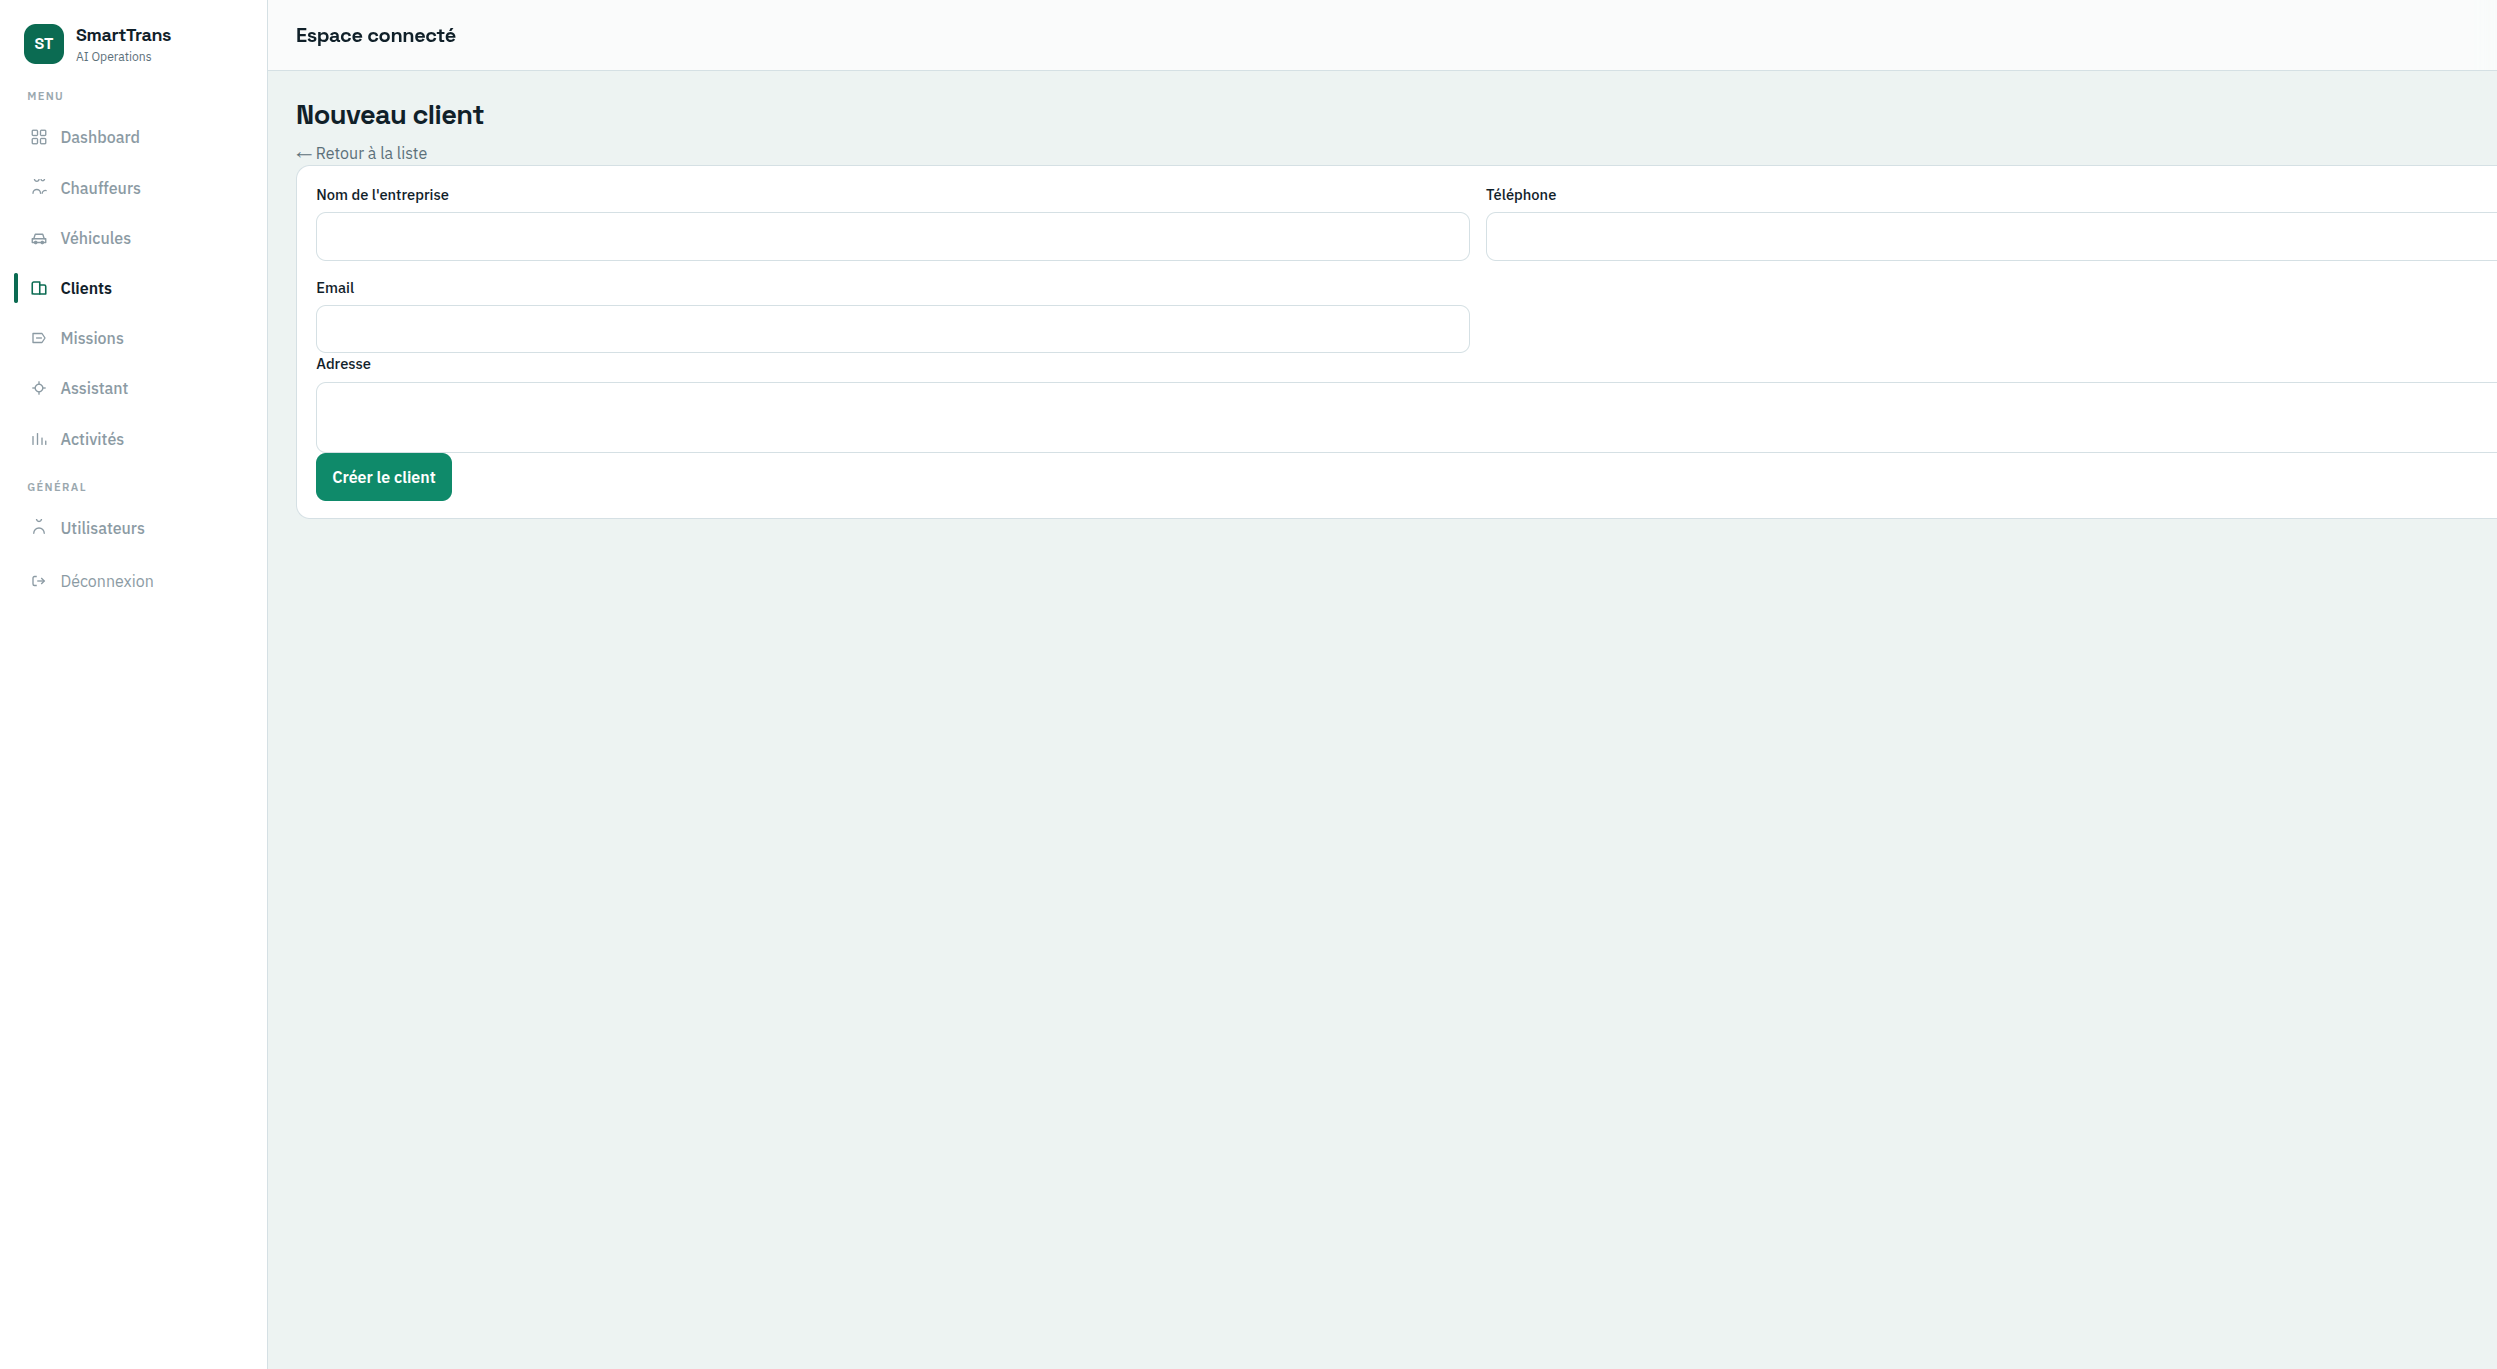
\includegraphics[width=0.88\textwidth,keepaspectratio]{ui-11-client-nouveau.png}
\caption{Formulaire de création d'un client}
\label{fig:ui-cli-new}
\end{figure}

\begin{figure}[htbp]
\centering
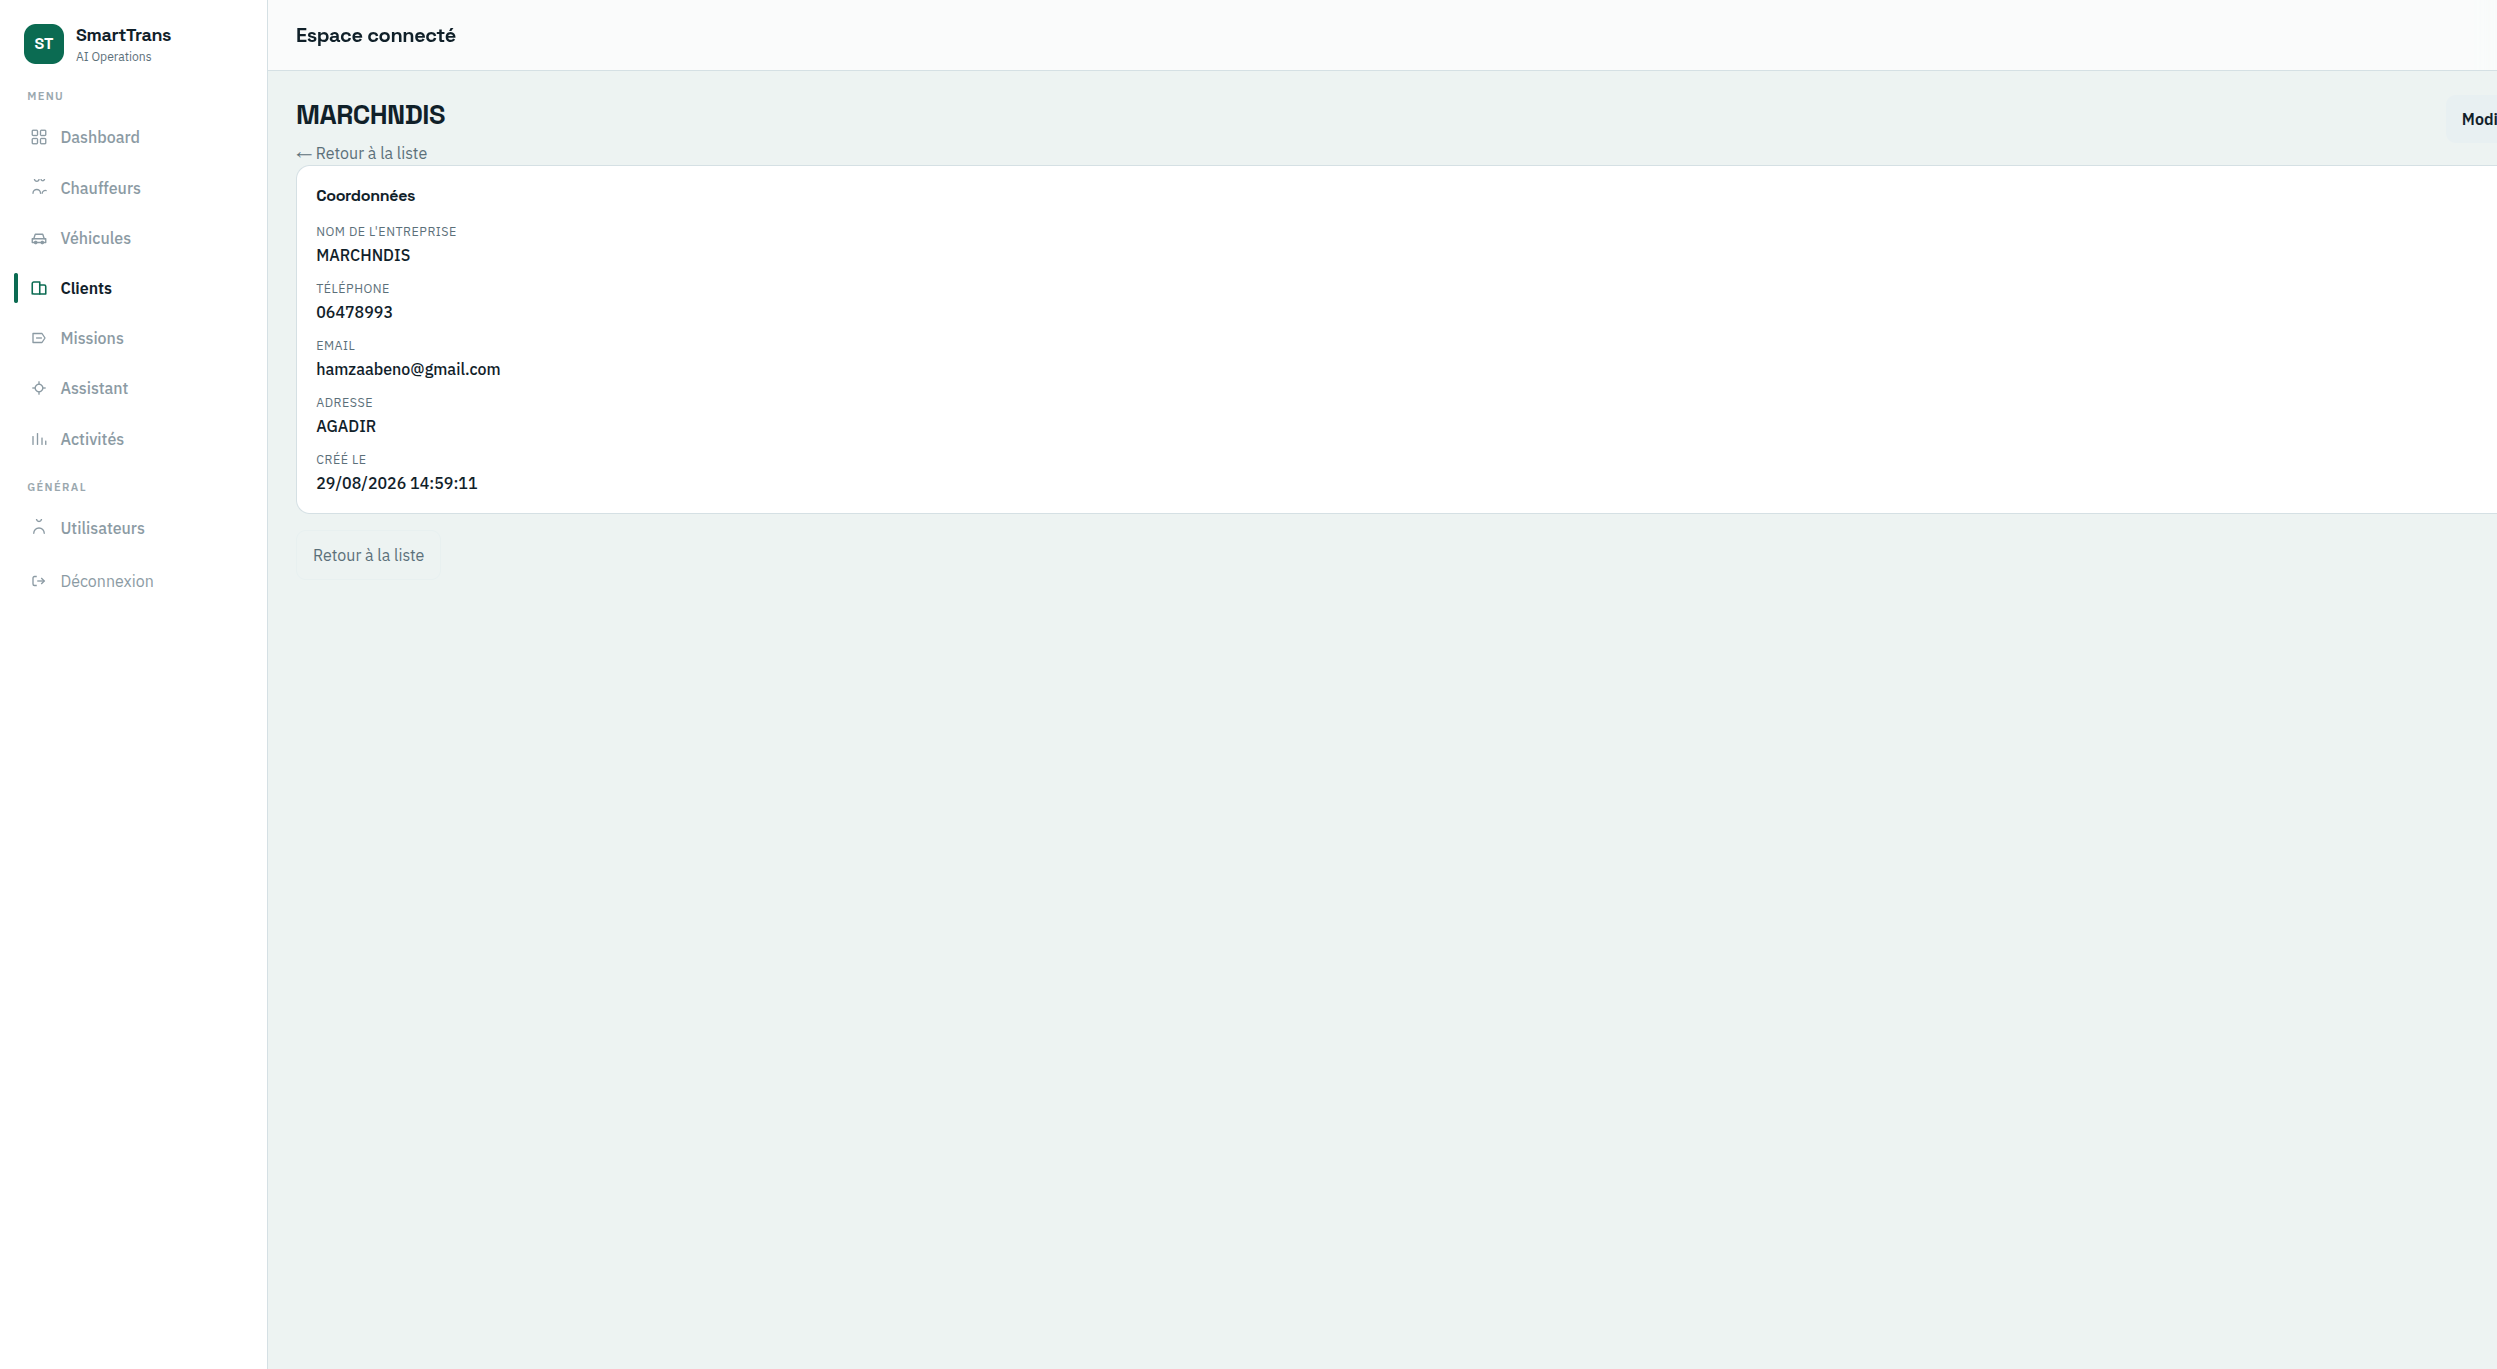
\includegraphics[width=0.88\textwidth,keepaspectratio]{ui-12-client-detail.png}
\caption{Fiche détail d'un client}
\label{fig:ui-cli-det}
\end{figure}

\section{Planification et suivi des missions}

La liste (figure~\ref{fig:ui-mis-list}) relie référence, client, trajet, date, chauffeur, véhicule et statut. Le formulaire de création (figure~\ref{fig:ui-mis-new}) impose une référence, un client et un trajet ; chauffeur et véhicule peuvent rester non assignés. Le détail (figure~\ref{fig:ui-mis-det}) montre l'état d'avancement et les dates de démarrage et de clôture.

\begin{figure}[htbp]
\centering
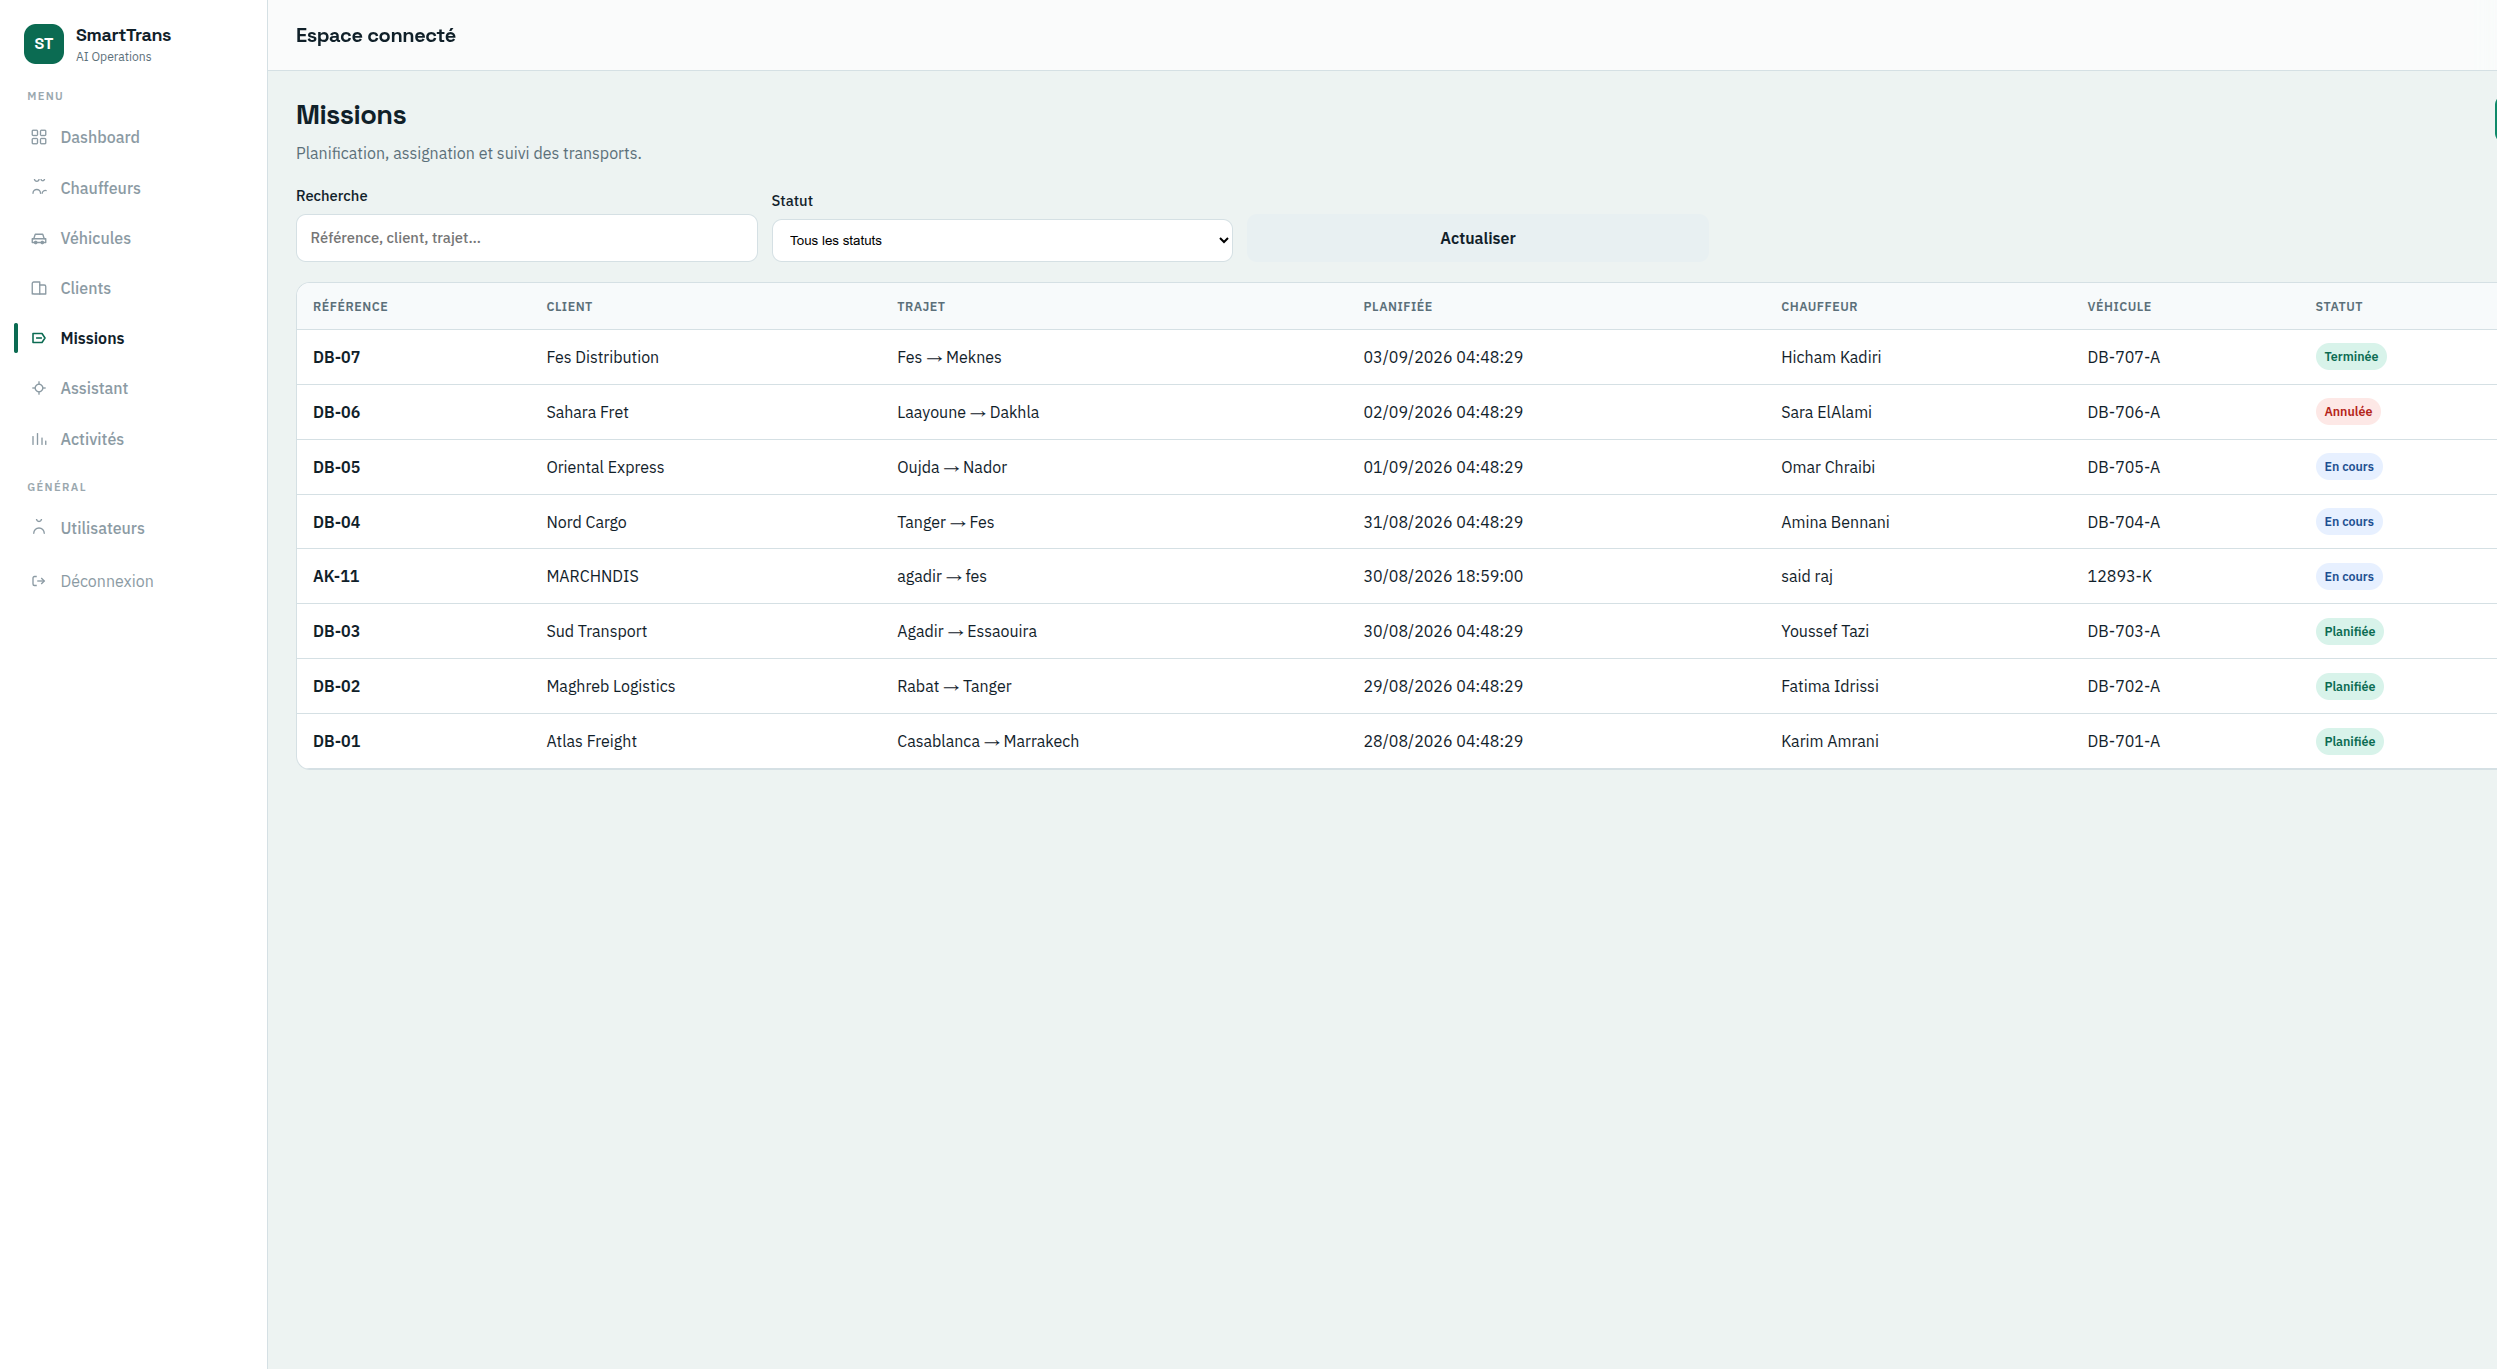
\includegraphics[width=0.95\textwidth,keepaspectratio]{ui-13-missions.png}
\caption{Liste des missions}
\label{fig:ui-mis-list}
\end{figure}

\begin{figure}[htbp]
\centering
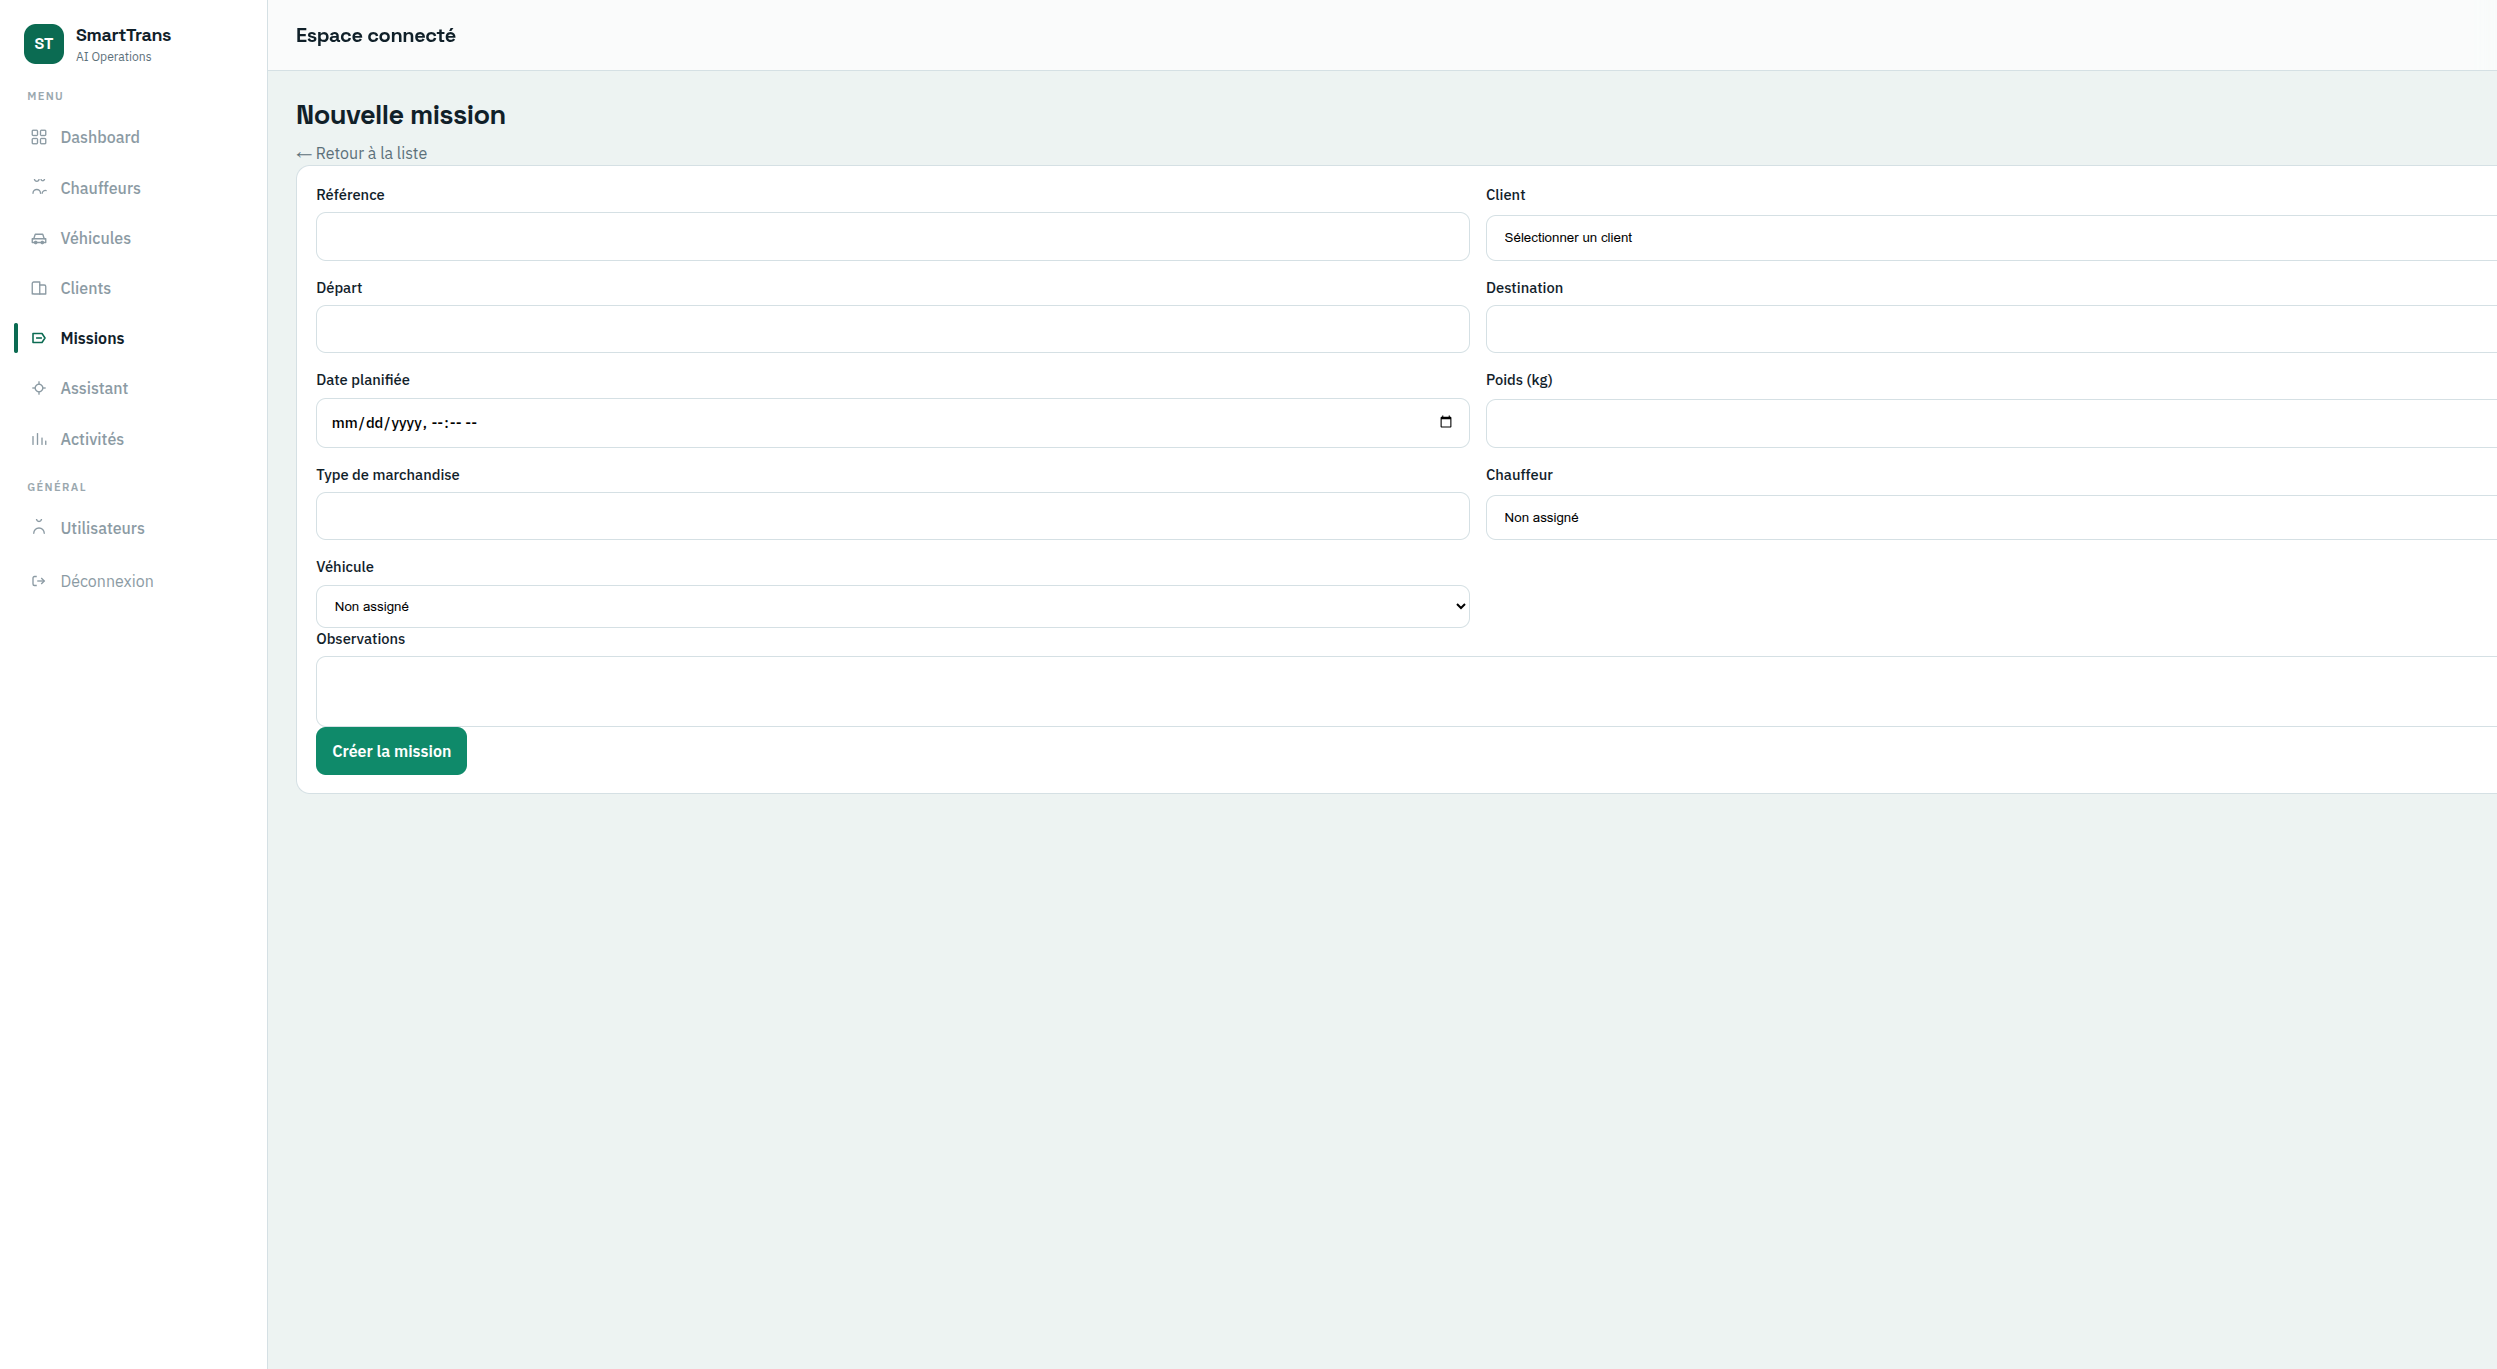
\includegraphics[width=0.88\textwidth,keepaspectratio]{ui-14-mission-nouvelle.png}
\caption{Formulaire de création d'une mission}
\label{fig:ui-mis-new}
\end{figure}

\begin{figure}[htbp]
\centering
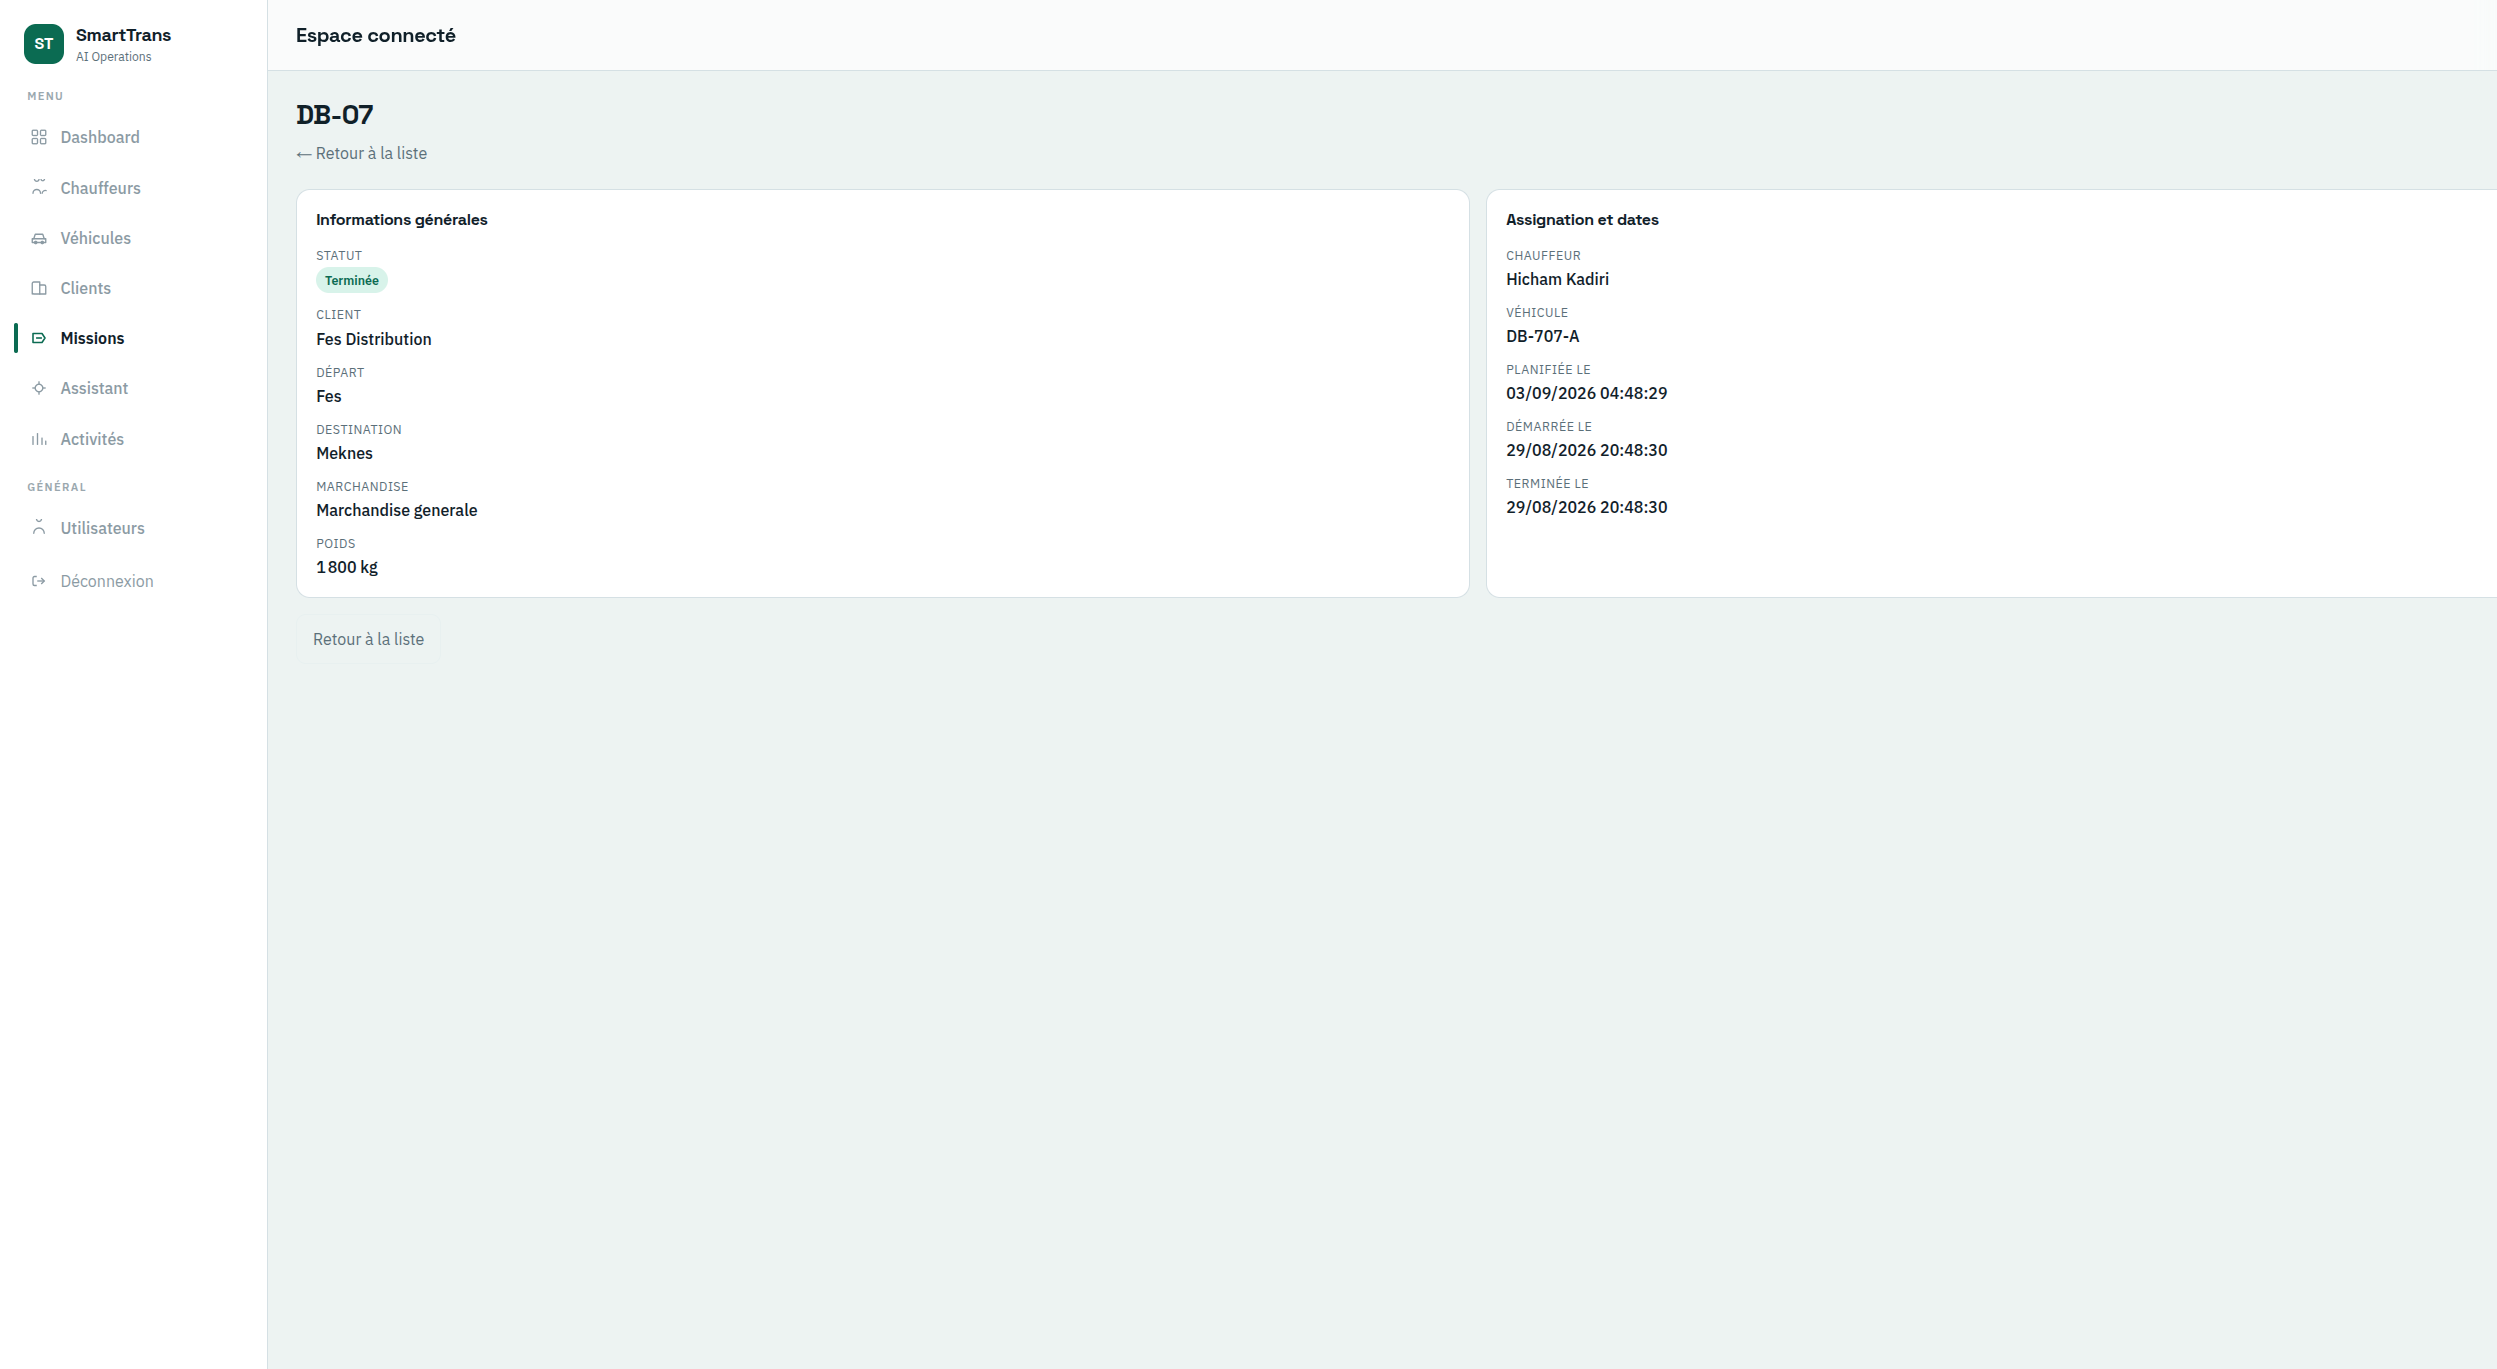
\includegraphics[width=0.88\textwidth,keepaspectratio]{ui-15-mission-detail.png}
\caption{Fiche détail d'une mission}
\label{fig:ui-mis-det}
\end{figure}

\section{Assistant}

La figure~\ref{fig:ui-ai} montre l'assistant réservé à l'exploitation. L'utilisateur pose une question en langue naturelle ou choisit une suggestion. La réponse s'appuie sur les données de la base (missions, chauffeurs, véhicules, alertes), afin de limiter les inventions.

\begin{figure}[htbp]
\centering
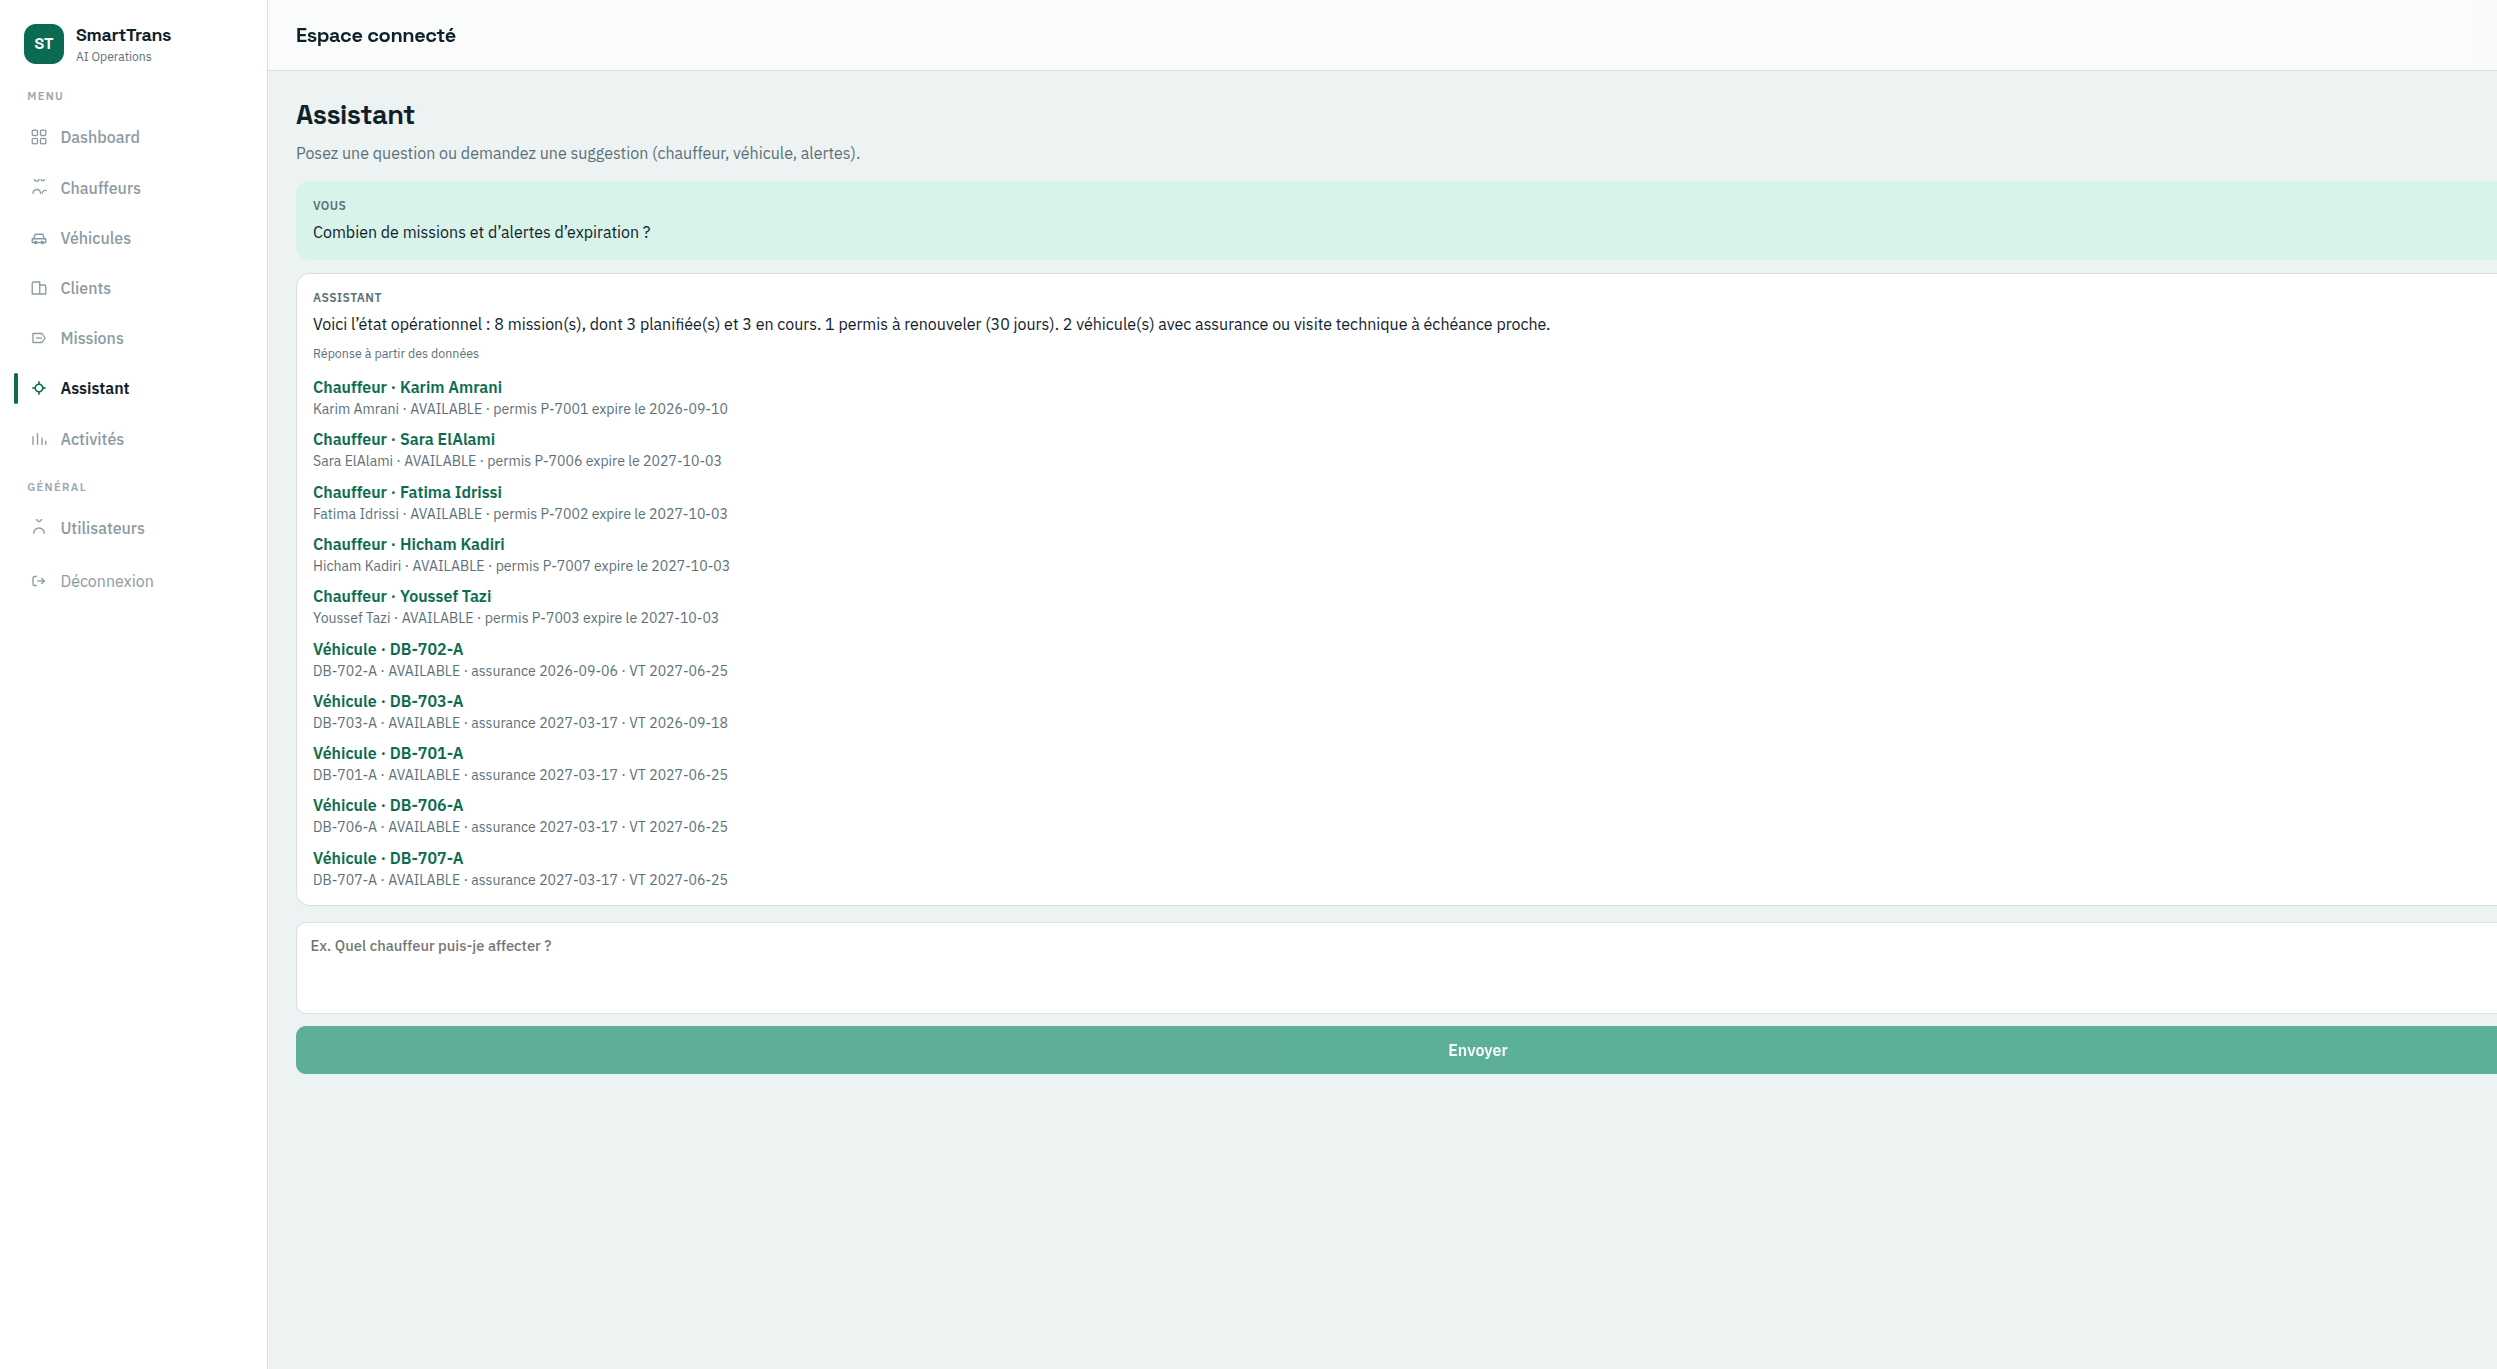
\includegraphics[width=0.95\textwidth,keepaspectratio]{ui-16-assistant.png}
\caption{Assistant conversationnel ancré sur les données métier}
\label{fig:ui-ai}
\end{figure}

\section{Journal d'activités}

La figure~\ref{fig:ui-act} présente le journal en lecture seule. Chaque ligne indique la date, l'action, le type d'entité et un libellé d'objet (courriel, référence de mission, nom, immatriculation). Le filtre par type d'action facilite l'audit.

\begin{figure}[htbp]
\centering
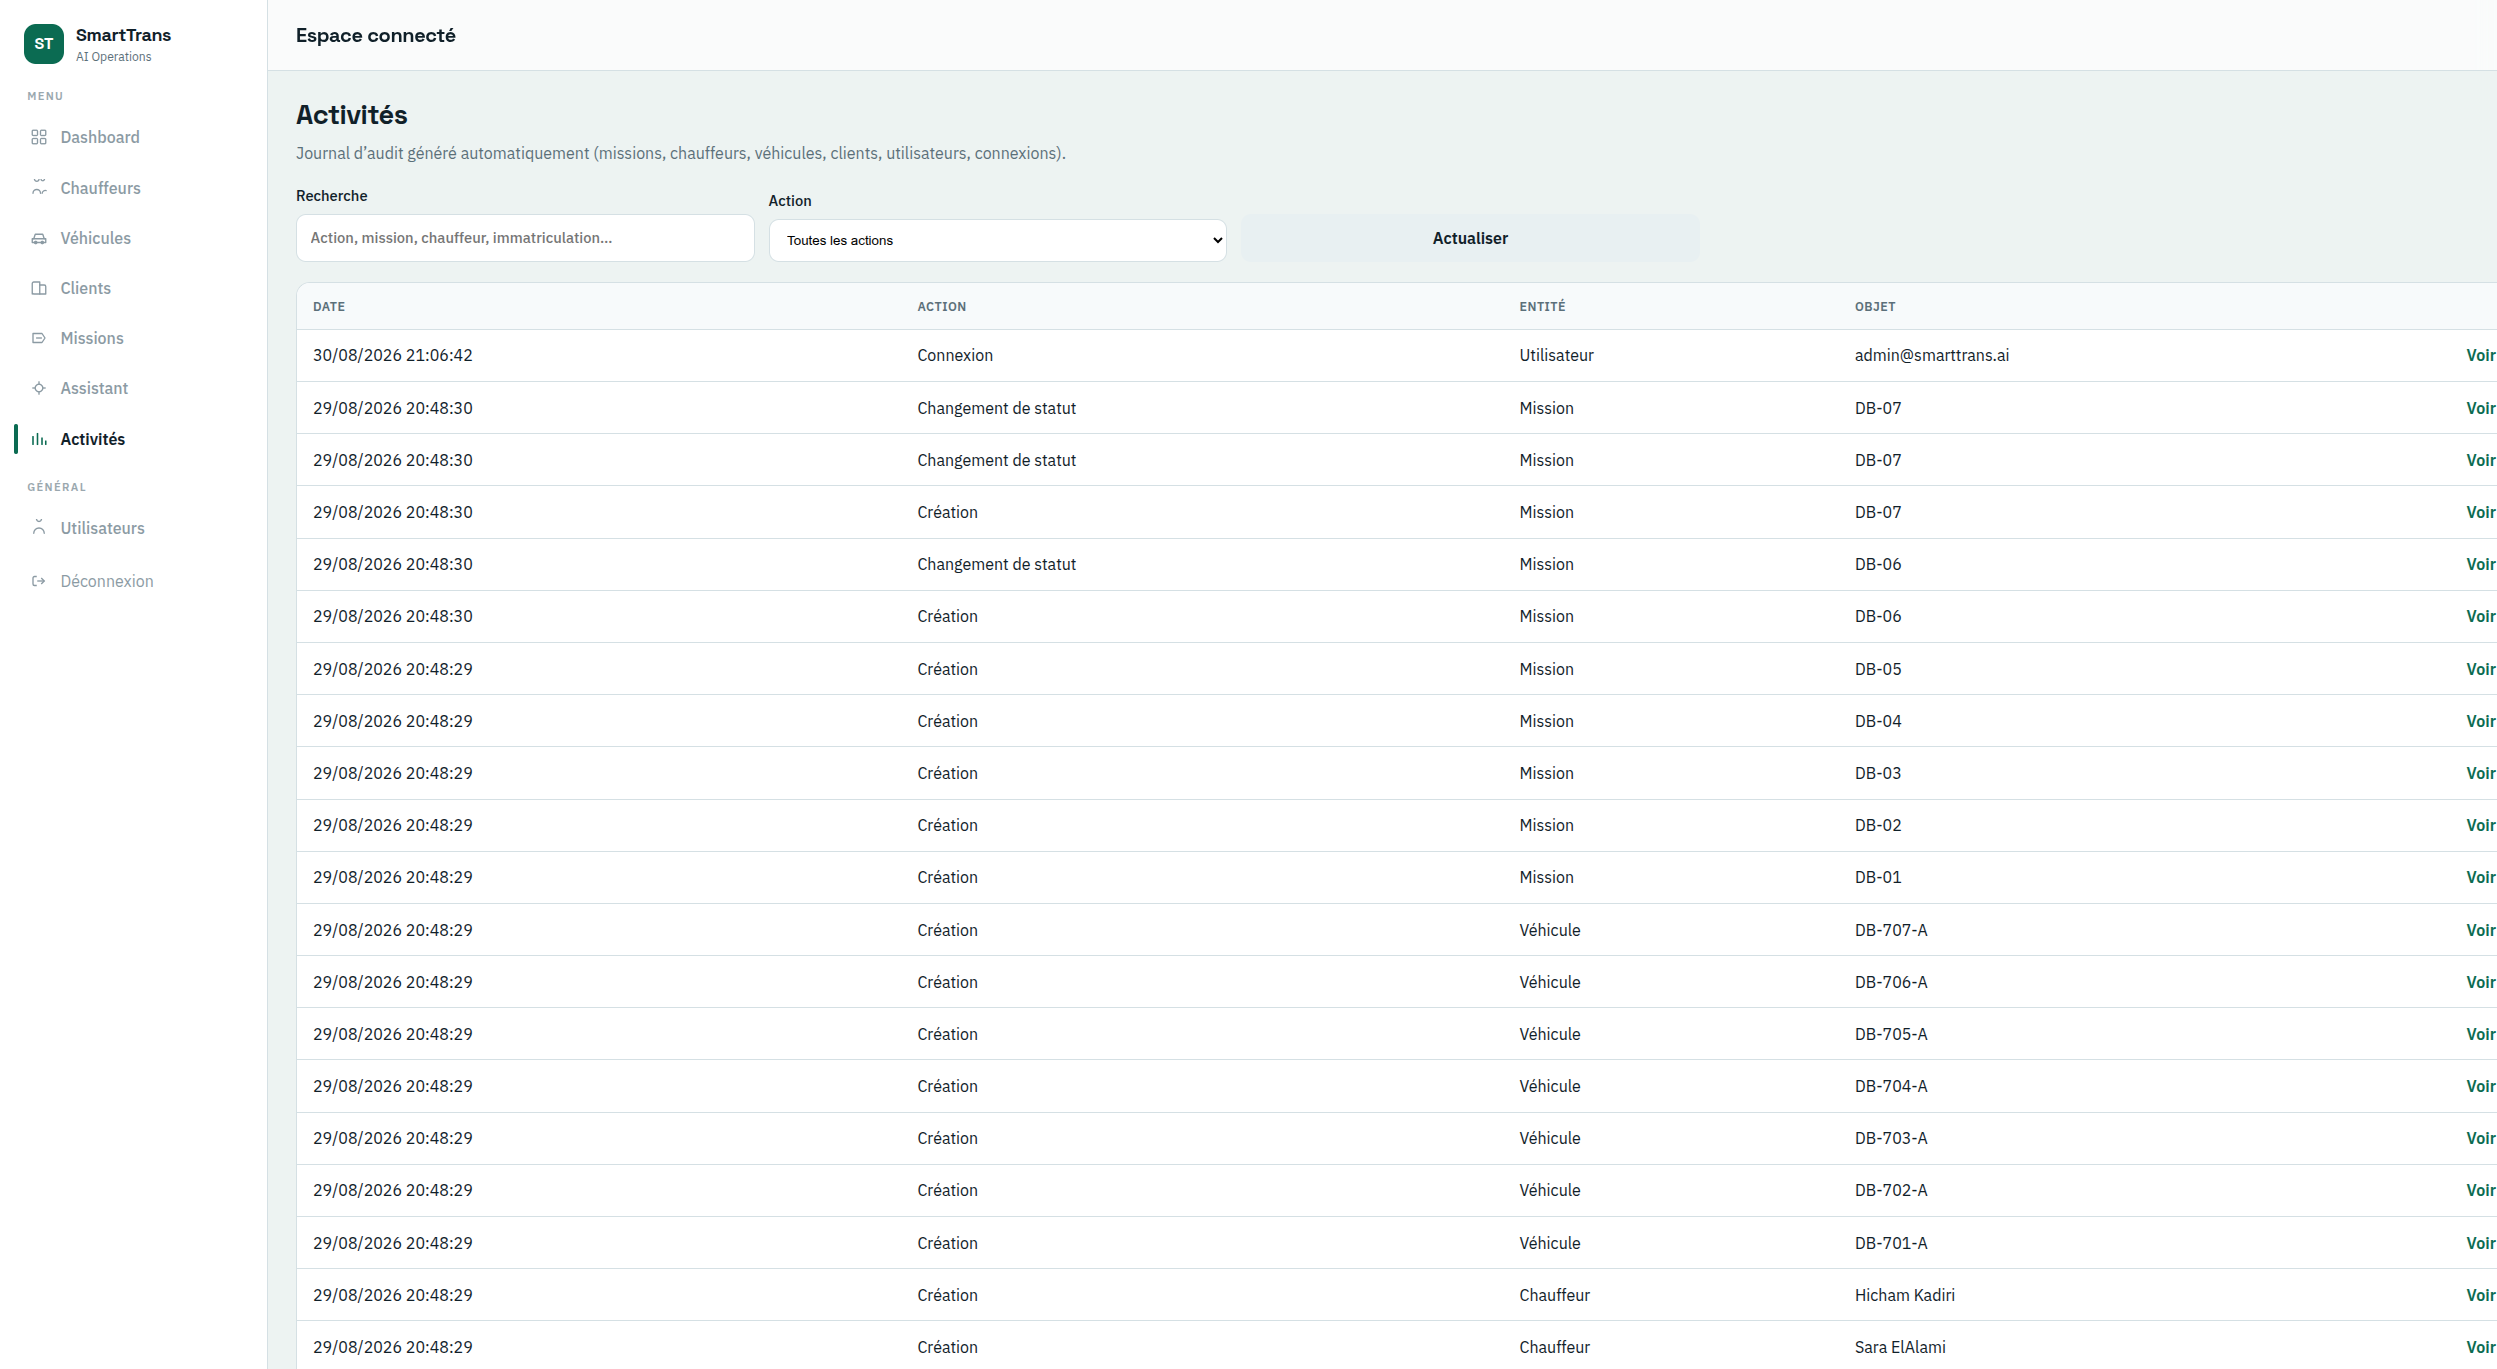
\includegraphics[width=0.95\textwidth,keepaspectratio]{ui-17-activites.png}
\caption{Journal d'activités (audit automatique)}
\label{fig:ui-act}
\end{figure}

\section{Administration : utilisateurs et rôles}

La liste des comptes (figure~\ref{fig:ui-usr}) et le formulaire de création (figure~\ref{fig:ui-usr-new}) sont réservés à l'administrateur. Les rôles (figure~\ref{fig:ui-rol}) correspondent aux trois profils du système : administrateur, responsable transport, chauffeur.

\begin{figure}[htbp]
\centering
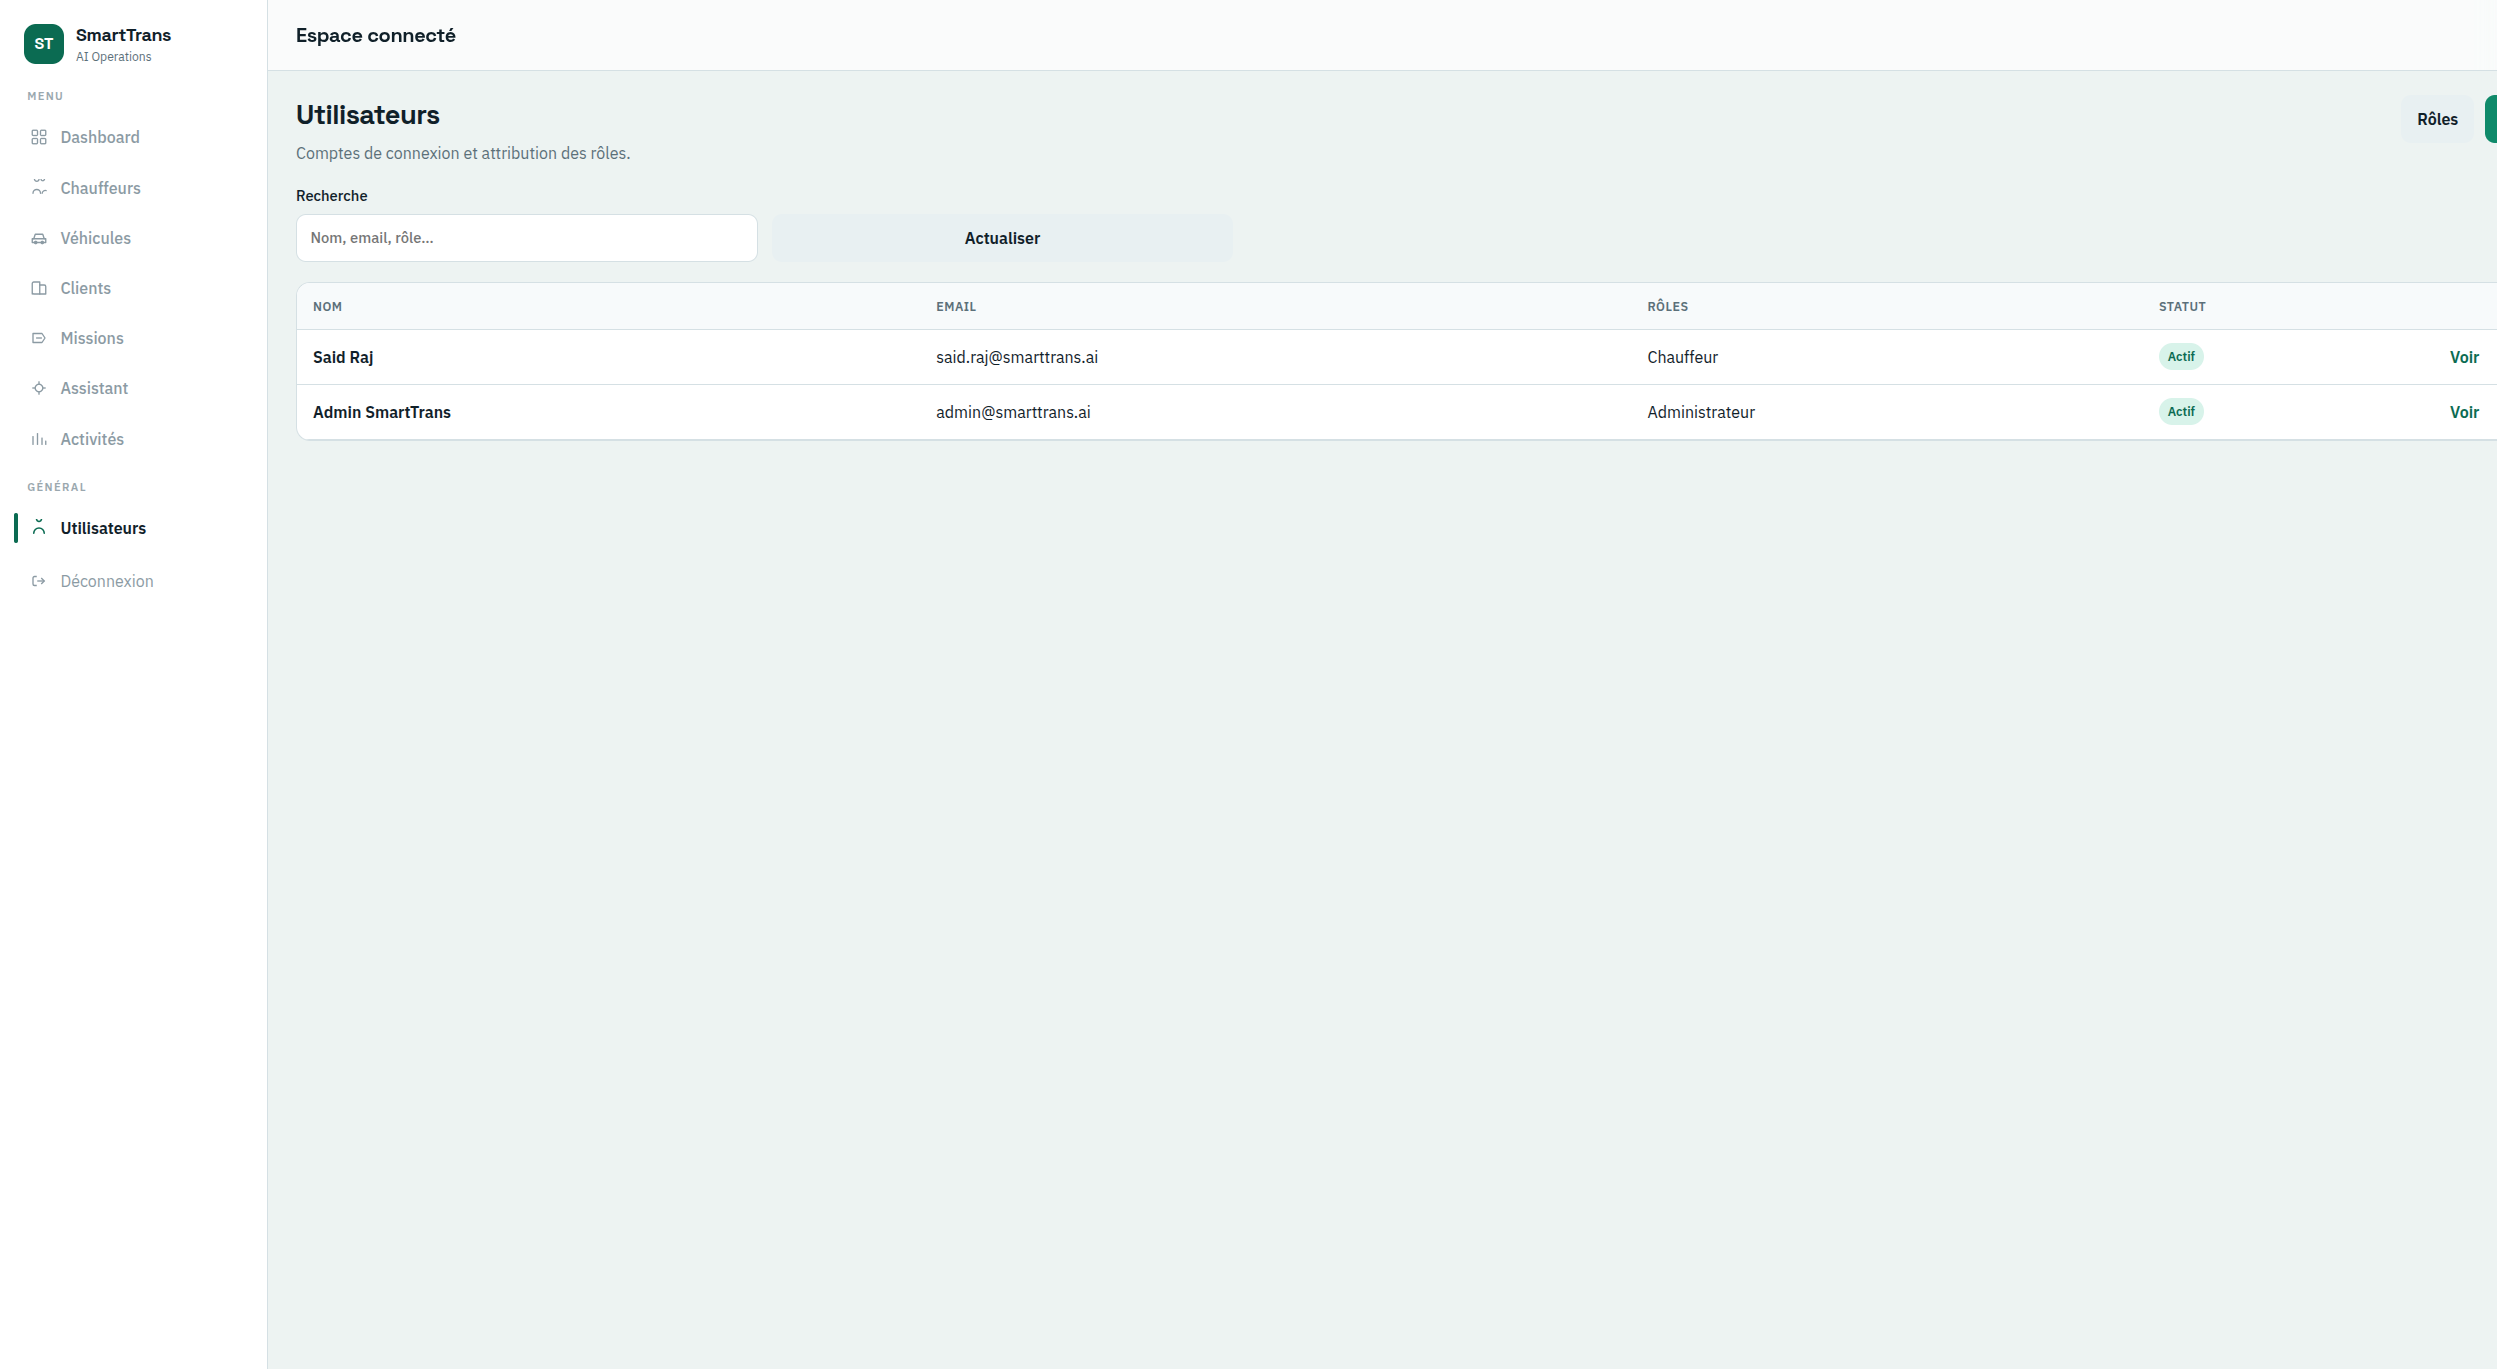
\includegraphics[width=0.95\textwidth,keepaspectratio]{ui-18-utilisateurs.png}
\caption{Liste des utilisateurs}
\label{fig:ui-usr}
\end{figure}

\begin{figure}[htbp]
\centering
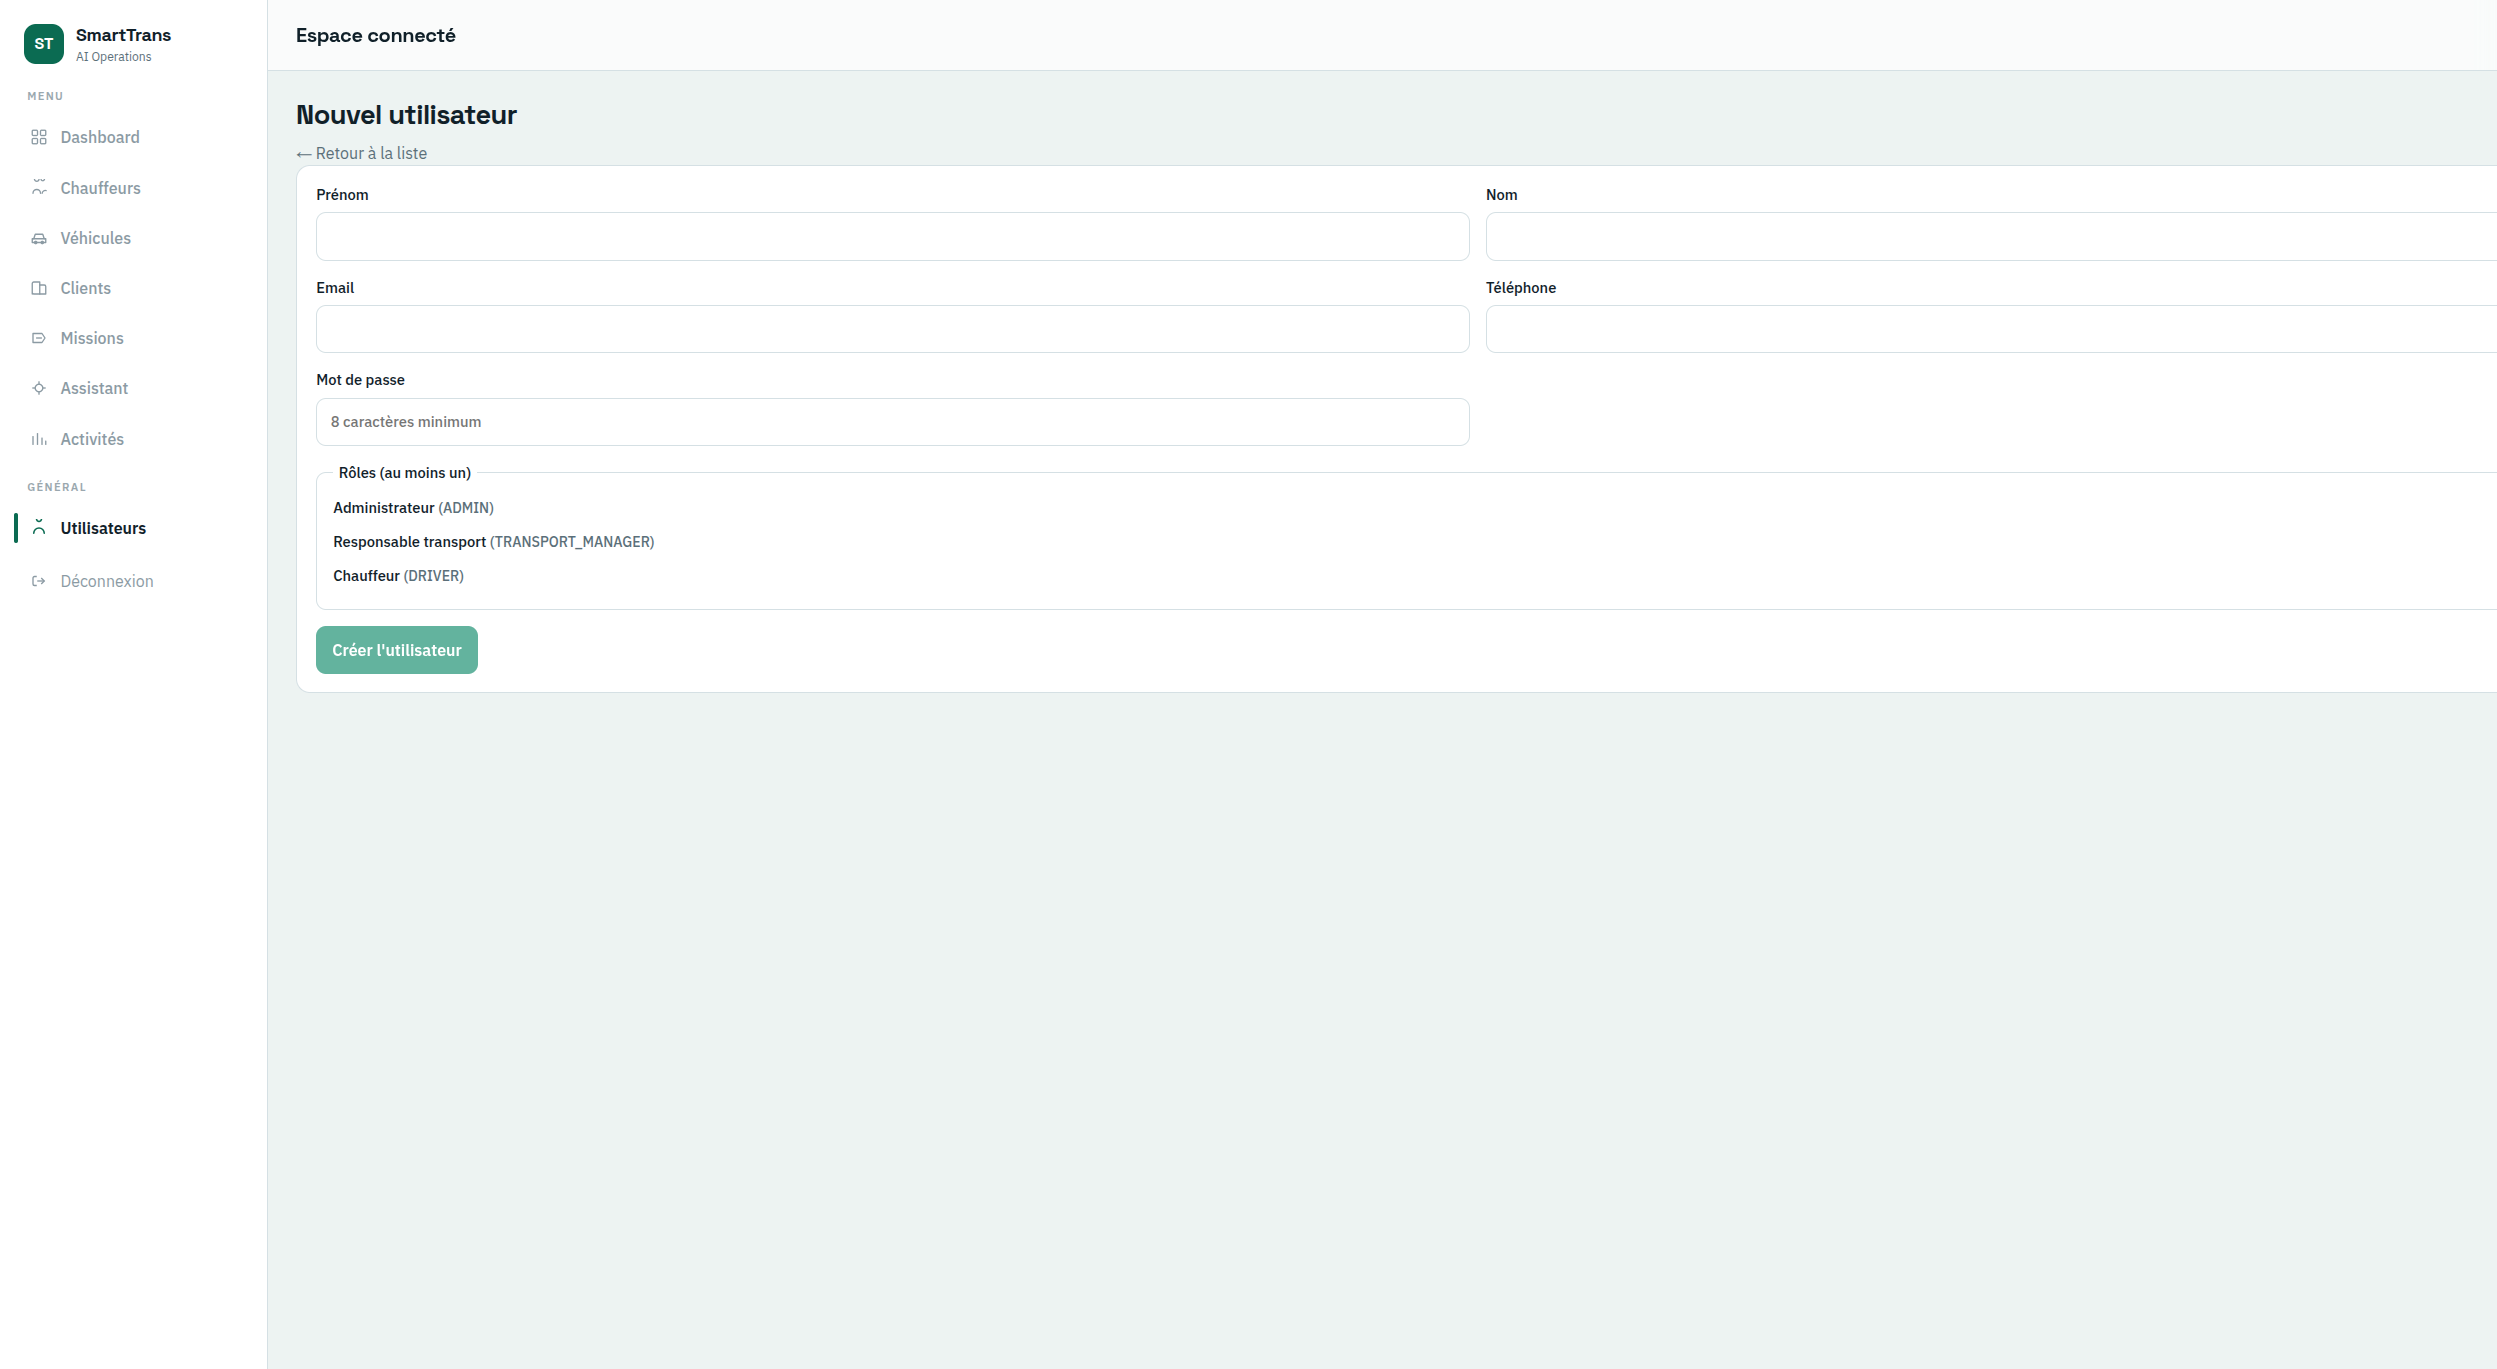
\includegraphics[width=0.88\textwidth,keepaspectratio]{ui-20-utilisateur-nouveau.png}
\caption{Formulaire de création d'un utilisateur}
\label{fig:ui-usr-new}
\end{figure}

\begin{figure}[htbp]
\centering
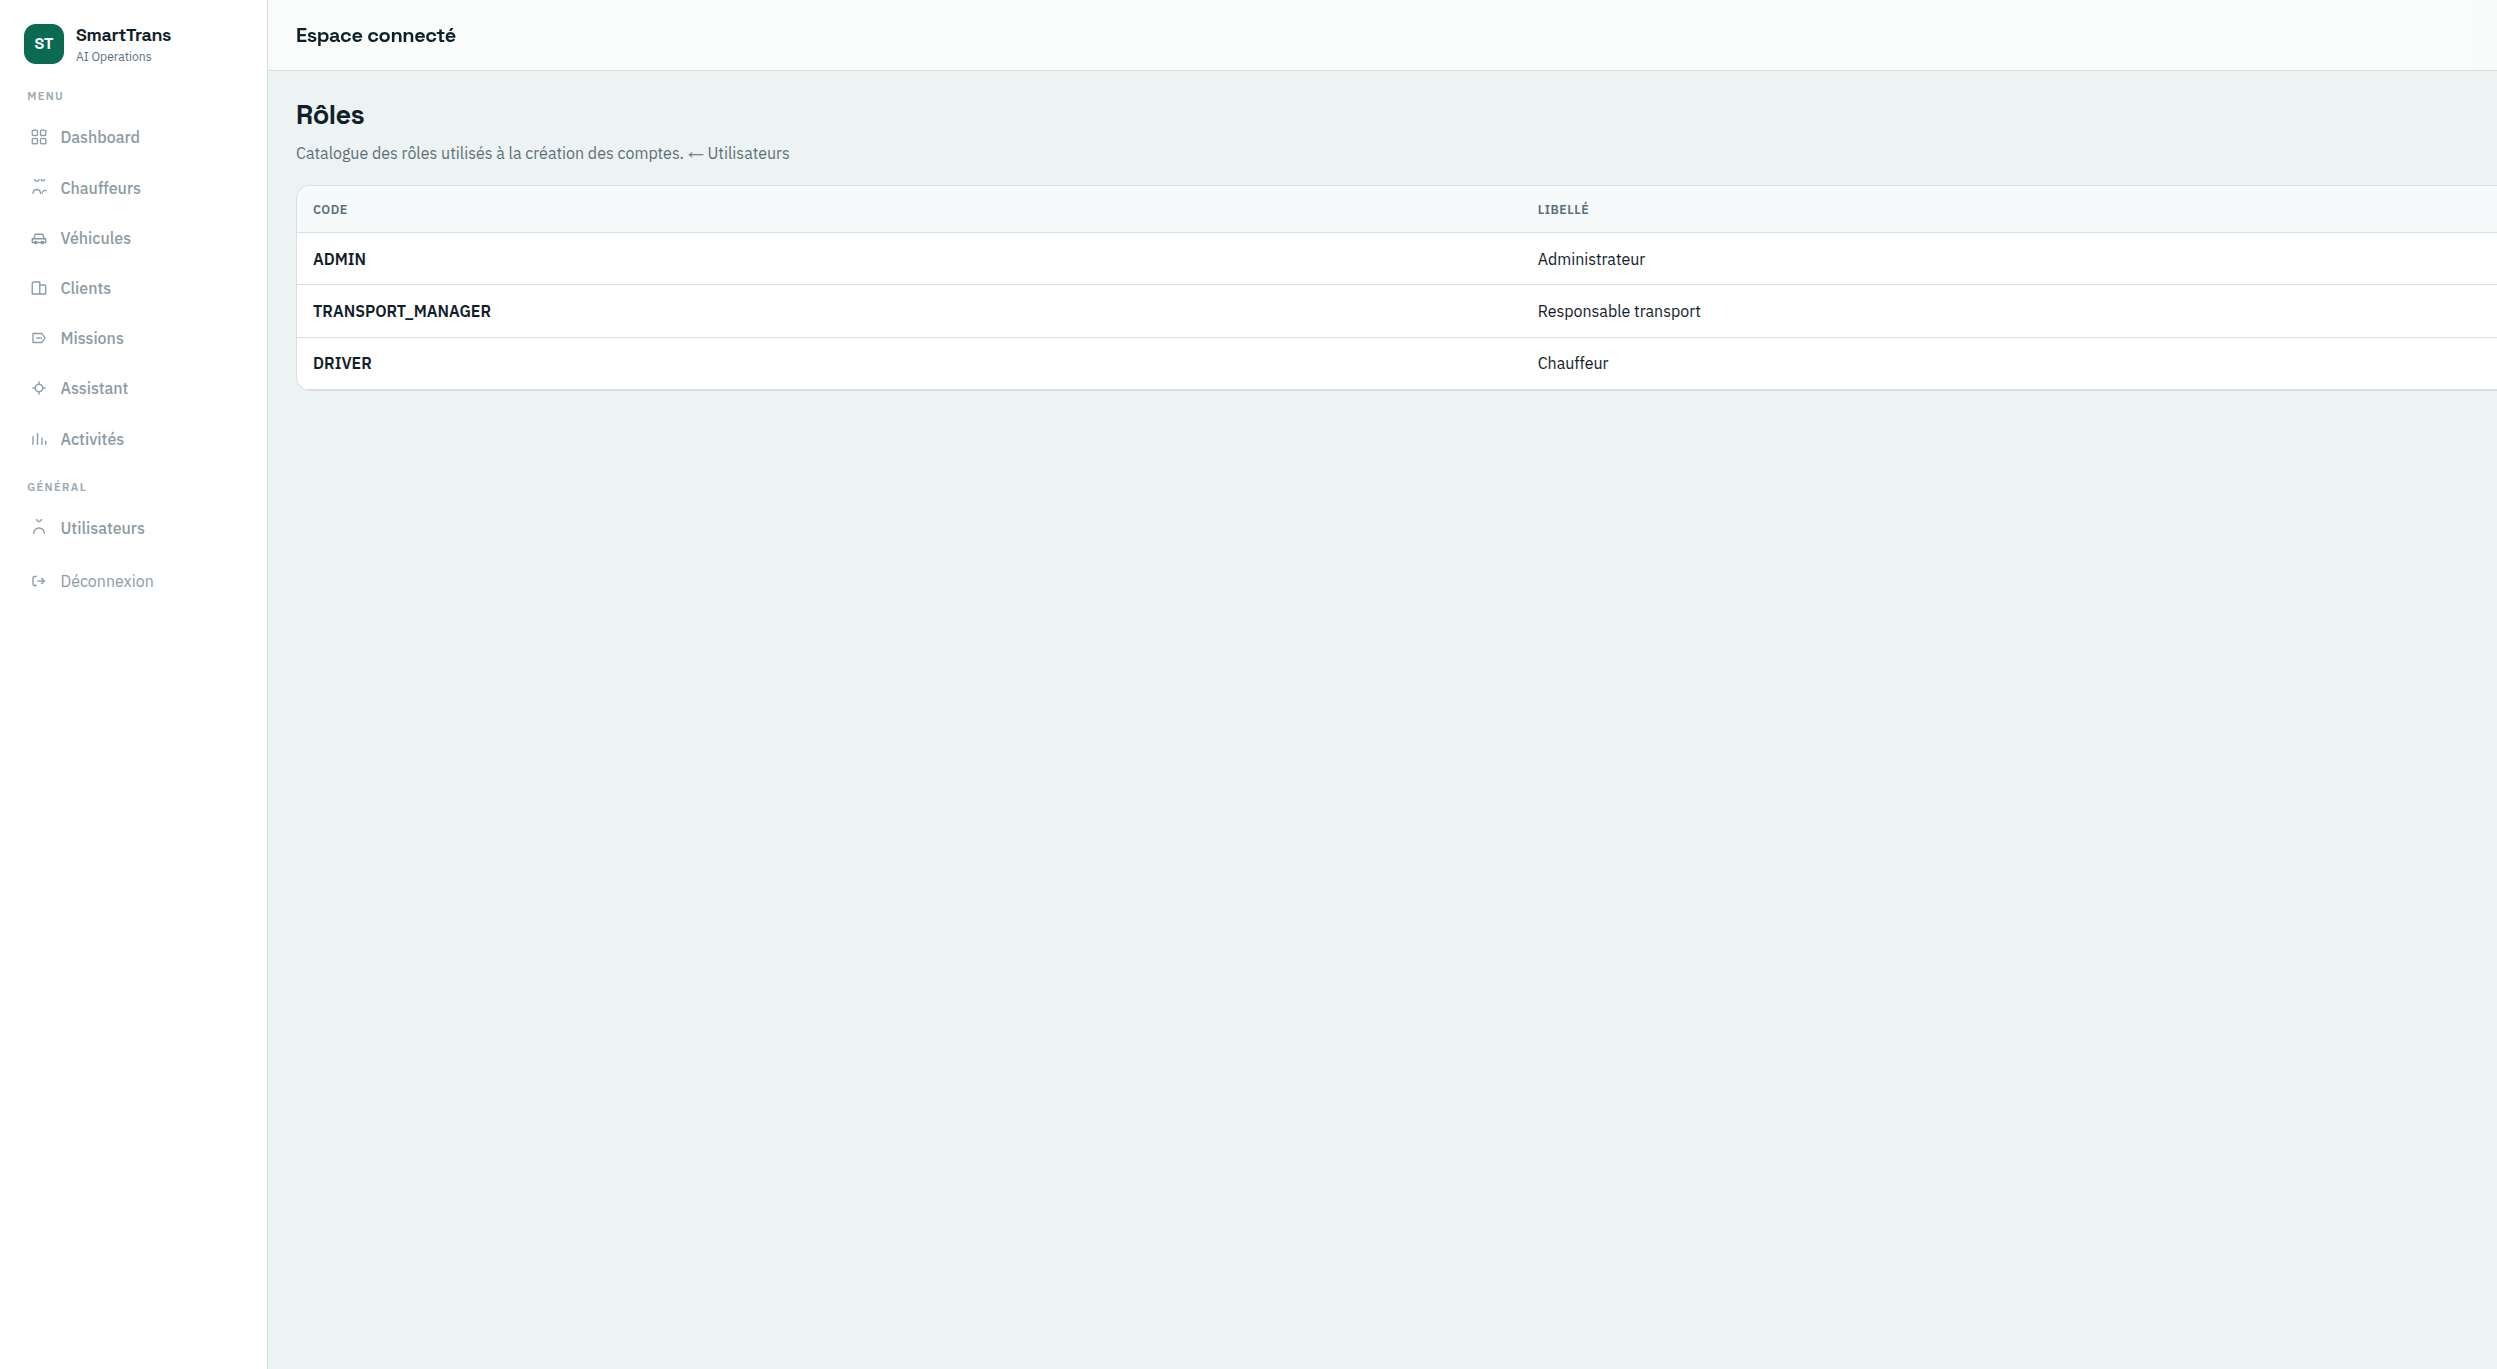
\includegraphics[width=0.88\textwidth,keepaspectratio]{ui-19-roles.png}
\caption{Catalogue des rôles}
\label{fig:ui-rol}
\end{figure}

\section{Conclusion}

Les captures confirment la cohérence de l'interface avec l'analyse : navigation par rôle, formulaires alignés sur le modèle de données, tableau de bord orienté alertes, assistant et journal pour le pilotage. La conclusion générale dresse le bilan du stage.
